\documentclass[a4paper,fleqn,usenatbib]{mnras}

%=========================================================================
\usepackage{amsmath} 
\usepackage{amssymb} 
\usepackage{multirow}

\usepackage{graphicx}
\usepackage{grffile}
\usepackage[dvips]{epsfig}
\usepackage{epsfig}  
\usepackage{color}
\usepackage{caption}
\usepackage{hyperref}
\usepackage{bm}
%Non reposionated tables

%=========================================================================
%		INTERNAL MACROS
%=========================================================================
\def\be{\begin{equation}}
\def\ee{\end{equation}}
\def\ba{\begin{eqnarray}}
\def\ea{\end{eqnarray}}

% To highlight comments 
\definecolor{red}{rgb}{1,0.0,0.0}
\newcommand{\red}{\color{red}}
\definecolor{darkgreen}{rgb}{0.0,0.5,0.0}
\newcommand{\SRK}[1]{\textcolor{darkgreen}{\bf SRK: \textit{#1}}}
\newcommand{\SRKED}[1]{\textcolor{darkgreen}{\bf #1}}
\newcommand{\before}[1]{\textcolor{red}{ #1}}
\newcommand{\after}[1]{\textcolor{darkgreen}{ #1}}
\newcommand{\hs}{{\hspace{1mm}}}  
\newcommand{\tol}{Tololo 1214-277}
\newcommand{\rank}{\texttt{Ranked}}
\newcommand{\boot}{\texttt{Bootstrapped}}
\newcommand{\rand}{\texttt{Random}}
\newcommand{\HI}{{\text{H\MakeUppercase{\romannumeral 1}}} }
\newcommand{\HII}{{\text{H\MakeUppercase{\romannumeral 2}}} }
\newcommand{\lya}{\ifmmode{{\rm Ly}\alpha}\else Ly$\alpha$\ \fi}
\newcommand{\cm}{\ifmmode{{\rm cm}}\else cm\fi}
\newcommand{\ccm}{\,\mathrm{cm}^{-3}}
\newcommand{\ergps}{\,{\rm erg}\,{\rm s}\ifmmode{}^{-1}\else ${}^{-1}$\fi}
\newcommand{\Mpch}{\,{\rm Mpc}\,\ifmmode h^{-1}\else $h^{-1}$\fi}
\newcommand{\dd}{\mathrm{d}}
\newcommand{\vek}[1]{\bm{#1}}
\newcommand{\hb}{H$\beta$}
\newcommand{\ha}{H$\alpha$}
\newcommand{\oiii}{[OIII]}
\newcommand{\oii}{[OII]}
\newcommand{\nii}{[NII]}
\newcommand{\esca}{erg cm$^{-2}$ s$^{-1}$ \AA$^{-1}$}
\newcommand{\esc}{erg cm$^{-2}$ s$^{-1}$}
\newcommand{\es}{erg s$^{-1}$}
\newcommand{\esa}{erg s$^{-1}$}
\newcommand{\kms}{\ifmmode\mathrm{km\ s}^{-1}\else km s$^{-1}$\fi}
\newcommand{\hMsun}{{\ifmmode{h^{-1}{\rm{M_{\odot}}}}\else{$h^{-1}{\rm{M_{\odot}}}$}\fi}}
\newcommand{\Msun}{{\ifmmode{{\rm{M_{\odot}}}}\else{${\rm{M_{\odot}}}$}\fi}}

\newcommand{\jefr}[1]{\textcolor{darkgreen}{\bf JEFR: \textit{#1}}}

\begin{document}

%=========================================================================
%		FRONT MATTER
%=========================================================================
\title[LG satellites distribution asphericity]{We are not the 99 percent: quantifying
  asphericity in the distribution of Local Group satellites}
\author[J.E. Forero-Romero \& V. Arias]
{Jaime E. Forero-Romero $^{1}$ \thanks{je.forero@uniandes.edu.co},
Ver\'onica Arias$^1$\\
%%
$^1$ Departamento de F\'isica, Universidad de los Andes, Cra. 1
  No. 18A-10 Edificio Ip, CP 111711, Bogot\'a, Colombia \\
}

\maketitle

\begin{abstract}
We use numerical simulations to build an explicit probability
distribution for the asphericity in the satellite distribution around
galaxies similar to the Local Group (LG) in the Lambda Cold Dark
Matter (LCDM) paradigm. 
This allows us to estimate the atipicallity
of the satellite distributions in the LG even when the underlying
simulations do not have enough systems that fully resemble the LG.
We demonstrate the method using three different simulations:
Illustris-1,  Illustris-1-Dark and ELVIS. 
Detailed results differ greatly among the simulations, suggesting a
strong influence of resolution, simulated physics and criteria to select
LG pairs.
However, there are three common trends in these simulations. 
First, at most of $1\%$ the pairs are expected to have satellite
distributions with the same asphericity aas the Local Group; second,
between $38\%$ to $59\%$ of the pairs have a halo with a satellite
distribution as aspherical as in M31; and third, at most $2\%$ of the
pairs have a satellite distribution as planar as in the MW. 
The brightest satellites in M31 galaxy turn out to have a rather
typical distribution in the LCDM context, while the MW is atypical in
this respect.  
These results place the LG at the level of a $3\sigma$ outlier
in the LCDM paradigm. 
The approach presented here facilitates the comparison between
asphericity results from different numerical setups and choices to
select halo pairs in simulations, hopefully helping to clarify the
reasons behin the LG atipicallity in LCDM. 
\end{abstract}

\begin{keywords}Galaxies: halos --- Galaxies: statistics --- Dark
  Matter --- Methods: numerical  
\end{keywords}

\section{Introduction}

The spatial distribution of satellite galaxies around our Milky Way and the
M31 galaxy provides a stringent test for structure formation theories
in a explicit cosmological context. 
The presence of a Vast Polar Structure of satellites around the Milky
Way has been stablished in the last decade.
This structure is present in the $11$ brightest "classical" dwarf
galaxies and has been confirmed as fainter satellites have been
detected. 
In the case of M31,  observational studies have found a planar satellite
distribution in a subset of $15$ satellites out of an homogeneous
sample of $27$ satellites. 
However, taking into account the $11$ brightest satellites (as a
comparison with the MW) there does not seem to be any planar structure.

The question whether this kind of planar configurations are atypical
in the observable Universe cannot be properly addressed given the
current limits in observations. 
So far it has only been possible to contraint that $5\%$ of the
Milky-Way like galaxies in the Universe have two bright satellite
galaxies as is the case of the Milky Way and its Large and Small
Magellanic Clouds. 

However, the tipicallity of satellite distributions can be addressed
in simulations.
Most of the studies have been performed in the currently preferred
paradigm, which is based on a Cold Dark Matter cosmology in a expanding
Universe described by General Relativity including a Cosmological
Constant, the so-called Lambda Cold Dark Matter (LCDM).
The broad consensus is that these highly structured satellite distributions
are hard to find in simulations.  
There are still disagreements on the precise degree of atypicallity
and the conditions required to simulate satellite distributions closer 

Some studies have focused on the study of individual dark matter halos
that could host galaxies like the MW or M31, while some other studies
have tried to simulate the formation of galaxy pairs resembling both
the MW and M31.
The transition from studying individual halos to pairs has been
motivated by the hypotesis hat the location of the Local Group in
the cosmic web should play a determinant role in building up planar
satellite distributions through preferential alignments and accretions
histories of galaxies.

Studies of the Local Group in an explicit cosmological context have
also renewed the interest on performing constrained simulations that
could reproduce the observed large scale structure of the Universe,
This has also motivated the study of the two dominant galaxies in the 
Local Group as a pair in a cosmological context finding that the LG
itself has relatively uncommon kinematic configuration in the context
of LCDM and a strong preference to lie along filaments.


The aim of our work is to put together some of these pieces in a 
simple framework to quantify how atypical is the satellite
distribution found in the Local Group.
Some of the explicit characteristics we want to keep in our treatment
of the problem are the (i) cosmological context, (ii) the LG as a pair
of galaxies and (iii) a simple and robust description for the
satellites. 

The first condition constrains the kind of simulations we use. 
We either results from fully cosmological simulations or resimulations
of cosmological sub-volumes. 
The second condition constraints the kind of samples we want to
use. We build explicit samples of pairs that resemble the kinematic
structure of the MW and M31. 
The third condition motivates to only use the inertia tensor as a
description for the satellites positions, while droping any
information that might come from 3D velocities (high uncertainties) or
involved algorithms for plane fitting.  

Finally, to compute the odds of finding the LG satellite distributions 
in LCDM simulations, we do not make a direct search for the exact
observed values into simulations because, as we show in Section, the
LG is itself rare and we do not have enough simulated systems to
perform such a brute force solution. 
We also avoid this direct comparison for a second reason. 
We do not want to implicitly use either LCDM or observations as what
is considered normal or standard and compute the deviations from that
point. 
Our approach is different. 
We set as a point of reference an spherical satellite
distribution to quantify how both simulations and observations
deviate from the spherical distribution.
Simulations help us to construct an explicit probability distribution
for deviations from sphericity in LCDM.
Then we compute the odds of finding n satellite distributions that
deviates from sphericity as much as the LG does. 

In Section we list the sources of the observational and
simulated data to be used throughout the paper.
Next, in Section we describe the methods we use to quantify and
characterize the satellite distributions.
In section we present the results. 
In the discussion section we quantify the correlations between the main
plane properties as described by the simulations.
We use this results to quantify the degree of atipicality of the LG
and estimate the volume that has to probed in simulations in order to
find a pair with a satellite distribution as atipical as the LG. 
Finally, we summarize our conclusions in Section .


\section{Data samples}

\subsection{Observational Data}
\label{sec:obs}

We use three dimentional positions as reported by. 
The appendix includes the tables with the values we use in our
computations.
For each central galaxy we use the 15 brightest satellites within a
distance of $300$kpc to the central galaxy.
The satellites for the MW are: 
THe satellites for M31 are:



\subsection{Data from the Illustris project}
\label{sec:illustris}

We use publicly available data from the Illustris Project 
\citep{2014MNRAS.444.1518V}. 
This suite of cosmological simulations, performed using the quasi-Lagrangian
code AREPO \citep{2010MNRAS.401..791S}, followed the coupled evolution of dark 
matter and gas and includes parametrizations to account for the effects of
gas cooling, photoionization, star formation, stellar feedback, black
hole and super massive black hole feedback. 
The simulation volume is a cubic box of $75$ \Mpch\ on a side.
The cosmological parameters correspond to a $\Lambda$CDM cosmology
consistent with WMAP-9 measurements \citep{2013ApJS..208...19H}. 

We extract halo and galaxy information from the Illustris-1 and
Illustris-1-Dark simulations, the former simulation includes
hydrodynamics and star formation prescriptions while the latter only
includes dark matter physics.
These simulations have the highest resolution in the current release of the
Illustris Project.
Illustris-1 has $1820^3$ dark matter particles and $1820^3$ initial gas
volumen elements, while Illustris-1-Dark has $1820^3$ dark matter particles.
This corresponds to a dark matter particle mass of
$6.3\times 10^6$\Msun\ and a minimum mass for the baryonic volume
element of $8.0\times 10^7$\Msun for Illustris-1 and a dark matter
particle mass of $7.6\times 10^6$\Msun for Illustris-1-Dark.
In both simulations the dark matter gravitational softening is $1.4$
kpc.

We buid a sample of pairs that resemble the conditions in the LG.
To construct this sample we select from Illustris-1 all galaxies with an stellar
mass in the range $1\times10^{10}\Msun <M_{\star}<1.5 \times 10^{11}
\Msun$.
Then we select the pairs with the following conditions.

\begin{itemize}
\item For each galaxy $A$ we find its closest galaxy $B$, if galaxy $A$ is also
the closest to halo $B$, the two are considered as a pair. 
\item With $d_{AB}$ the distance between the two galaxies and
  $M_{\star,min}$ the lowest stellar mass in the two galaxies, we
  discard pairs that have any other galaxy $C$ with stellar mass
  $M_{\star}>M_{\star, min}$ closer than $3\times d_{AB}$ from any of
  the pair's members. 
\item The distance $d_{AB}$ is greater than $700$ kpc.
\item The relative radial velocity between the two galaxies, including
  the Hubble flow, is $-120\ \kms <v_{AB,r}<0\ \kms$. 
\end{itemize}

We find 27 pairs with these conditions. 
We then select the pairs where in both halos there are at least 15
detected subhalos, thus discarding pairs with halos with the lowest
mass.
We end up with a total of 20 pairs in Illustris-1.
In Illustris-1-DM we use the center of mass position of the 27 pairs
in Illustris-1 to find the matching halo pairs.
After discarding the pairs with less than 15 detected subhalos in one
of the halos we end up with a toal of 24 pairs. 
This corresponds to a pair number density of $\sim 2 \times10^{-5}$
pairs Mpc$^{-3}$ 
Appendix A shows the physical  properties (stellar masses, maximum
circular velocities, radial velocities and separation) in those
pairs.


Although Illustris-1 has stellar particles, we do not use their
properties to select the satelite population because the smallest
galaxies are barely resolved in stellar mass at magnitudes of
$M_V=-9$, close to the limit of the 11 ``classical'' MW satellites.
We use instead the dark matter information as the smallest sub-halos
we care about are sampled with at least $40$ particles.  

Both in Illustris-1 and Illustris-1-Dm we chose the satellite samples
by ranking the subhalos in decreasing order of its current maximum
circular velocity and select the first $N_p$ halos in the list.  
The results presented here correspond to $11\leq N_p\leq 15$. 

\subsection{Data from the ELVIS project}
\label{sim:ELVIS}



We use data from the public release of the Exploring the Local
Universe In Simulations (ELVIS) project.
For a detailed description of that project and its data we refer the
reader to \cite{XX}. 
Here we summarize the elements relevant to our discussion.

ELVIS data comes from resimulations of dark matter halo pairs selected
in dark matter only cosmological simulations. 
The parent cosmological boxes have a cosmology consistent with the
Wilkinson Microwave Anisotropy Probe 7 results.


The ELVIS project used the results from $50$ simulation boxes of side
lenght $70.4$ Mpc to select pairs with kinematic characteristics
similar to the LG. 
These selection criteria included the following
\begin{itemize}
\item The virial mass of each host must be in the range 
$1\times
  10^{12} M_{\odot}< M_{vir}<3\times 10^{12}M_{\odot}$ 
\item The total pair mass must be in the range
$2\times
  10^{12} M_{\odot}< M_{vir}<5\times 10^{12}M_{\odot}$ 
\item The center of mass separation is in the range $0.6\leq d\leq1$
  Mpc.
\item The relative radial velocity is negative.
\item No halos more massive than the least massive halo within $2.8$
  Mpc and no halos with $M_{vir}>7\times 10^{13}$ within $7$ Mpc of
  the pairs' center of mass.
\end{itemize} 

This corresponds to a pair number density of $\sim 8 \times10^{-6}$ pairs
Mpc$^{-3}$, this is a factor $\sim 2.5$ lower than the pair number density
we find in the Illustris data.
There were a total of 146 pairs that met those criteria, but only $12$
were chosen for resimulation. 
Additionally, the selected pairs for resimulation have a relative
tangential velocity less than $75$ \kms. 
The dark matter particle resolution in these resimulations is
$1.9\times 10^5$, a thousand times larger than Illustris-1.
In this paper we only use the results from these $12$ resimulated pairs.

Appendix A compares the physical properties (stellar masses, maximum
circular velocities, radial velocities and separation) in those
pairs against the results from the Illustris-1 simulations.

\section{Building, Characterizing and Comparing Satellites Spatial Distributions}
\label{sec:SpatialMeasurements}


\subsection{Building Satellite Samples}

We compare the joint satellite distributions in the MW and M31 at fixed
satellite number, $N_s$.
This means that the magnitude cut corresponding to the faintest
satellite included in the sample is different in each case.
We make this choice for two reasons. 
First, to be sure that there is a non-zero number of satellites in the
simulations to make the computations.  
Second, to rule out the influence of satellite numbers in the
statistics. 

We compute the satellite statistics fo 11 up to 15 satellites.
The lowest bound corresponds to the number of classical Milky Way
satellites.
The upper limit corresponds to the maximum number of satellites that
can be resolved in both halos for most of the isolated pairs in Illustris-1.
In simulations we rank the subhalos by their maximum
circular velocity, in observations we rank the satellites by its $M_V$
magnitude. 

We also use two kinds of satellite distributions. 
The first keeps the positions for the satellites fixed as provided in
the observations/simulations; the second randomizes the angular positions of
the satellites around the central galaxy while keeping its radial
distance fixed. The randomization process is done 1000 times for each
galaxy. 



\begin{table*}
  \centering
  \renewcommand{\arraystretch}{1.2}
  \begin{tabular}{|p{2.5cm}|c|c|c|c|}
    \hline
    \multirow{2}{4.0cm}{} & \multicolumn{2}{c|}{\textbf{Observations}} & \multicolumn{2}{c|}{\textbf{Randomized Obs.}} \\
    % \hline
    % \textbf{Inactive Modes} & \textbf{Description}\\
    \cline{2-5}
    & \textbf{M31} & \textbf{MW} & \textbf{M31} & \textbf{MW} \\
    %\hhline{~--}
    \hline
    Plane width (kpc) & $59\pm 3$  & $22\pm 2$  & $64\pm 12$   & $45\pm 8$    \\\hline
    $c/a$ ratio & $0.45\pm 0.04$ & $0.28\pm 0.03$ & $0.55\pm0.10$ & $0.53\pm 0.10$ \\ \hline
    $b/a$ ratio & $0.82\pm 0.06$ & $0.78\pm 0.02$ & $0.82\pm0.07$ & $0.81\pm 0.08$ \\ \hline
  \end{tabular}
  \caption{Results from observations. Mean values and standard deviations for the different
    quantities describing satellite distribution: plane width, $c/a$
    ratio and $b/a$ ratio. 
    The first colum refers to the results from
    observational data, the second column uses the spherically
    randomized version of the observational data. \label{table:observations}}
\end{table*}


\begin{table*}
  \centering
  \renewcommand{\arraystretch}{1.2}
  \begin{tabular}{|p{2.5cm}|c|c|c|c|c|c|}
    \hline
    \multirow{2}{4.0cm}{} & \multicolumn{2}{c|}{\textbf{Illustris-1-Dark}} & \multicolumn{2}{c|}{\textbf{Illustris-1}} & \multicolumn{2}{c|}{\textbf{ELVIS}}\\
    % \hline
    % \textbf{Inactive Modes} & \textbf{Description}\\
    \cline{2-7}
    & \textbf{M31} & \textbf{MW} & \textbf{M31} & \textbf{MW}& \textbf{M31} & \textbf{MW}\\
    %\hhline{~--}
    \hline
    Plane width (kpc) & $62\pm 3$   & $61\pm 3$     & $70\pm 4$ & $67\pm 2$ & $70\pm 2$& $68\pm 4$ \\\hline
    $c/a$ ratio & $0.50\pm0.01$ & $0.50\pm 0.02$ & $0.52\pm 0.01$ & $0.53\pm 0.01$ & $0.54\pm 0.01$& $0.49\pm 0.02$ \\ \hline
    $b/a$ ratio & $0.79\pm0.01$ & $0.81\pm 0.02$ & $0.80\pm 0.01$ & $0.80\pm 0.02$ & $0.80\pm0.01$& $0.81\pm 0.01$\\ \hline
  \end{tabular}
  \caption{Results from simulations. Mean values and standard deviations for the different
    quantities describing satellite distributions: plane width, $c/a$
    ratio and $b/a$ ratio. 
    The first column summarize the results from the 24 pairs in
    Illustris-1-Dark, the second column from the 20 pairs in
    Illustris-1 and the third column from the 12 pairs in the
    ELVIS project.\label{table:simulations}}
\end{table*}



\subsection{Describing Samples with the Inertia Tensor}
We base all our results on the description provided by the inertia
tensor defined by the satellites's positions.  

\begin{equation}
{\bf{\bar{I}}} = \sum_{k=1}^{N_s}[(\bf{r}_i - \bf{r}_0)^2\cdot \bf{1} -
  (\bf{r}_i-\bf{r}_0)\cdot (\bf{r}_i - \bf{r}_0)^{T}],
\end{equation}
%
where $k$ indexes the set of satellites of interest
$\bf{r}_k$ are the satellites' positions, $\bf{r}_{0}$ is the location
of the central galaxy $\bf{1}$ is the unit matrix,  and  
${\bf r}^T$ is the transposed vector $\bf{r}$. 
We use $\bf{r}_0$ as the position of the central galaxy, and not the
satellites' geometrical center, to allow for a fair comparison once
the angular positions of the satellites are randomized around this
point. 

From this tensor we compute its eigenvalues,
$\lambda_1>\lambda_2>\lambda_3$, and corresponding eigenvectors,
$\hat{I}_1$, $\hat{I}_2$, $\hat{I}_3$.
We define the size of the three ellipsoidal axis as
$a=\lambda_1$, $b=\lambda_2$ and $c=\lambda_3$.
We also define $\hat{n}\equiv \hat{I}_1$ as the vector perpendicular to the
planar satellite distribution. 
We also define the width, $w$, of the planar satellite distribution,
as the standard deviation of all satellite distances to the plane
defined by the vector $\hat{n}$.  



To summarize we characterize the satellite distribution by for
quantities obtained from the inertia tensor: 
\begin{itemize}
\item Plane width, $w$.
\item $c/a$ axis ratio.
\item $b/a$ axis ratio.
\end{itemize}


\subsection{Comparing Satellite Samples}

We compare every satellite distribution against its own spherically
randomized distribution.
We keep fixed the radial position of every satellite
with respect to the central galaxy and then randomizing its angular
position. 
We repeat this procedure 1000 times for each satellite distribution
and proceed to measure the quantities mentioned in the last section:
$w$, $c/a$ and $b/a$.
For each quantity we compute an average and standard deviation from
the 1000 random samples. 
This allows us to build a normalized version of all quantities of
interest by substracting the mean and dividing between the standard
deviation of the randomized samples.

This allows us to make a first comparison. 
The observed/simulated
distribution against its randomized version. 
The second intermediate comparison we make are observations against
simulations.
The final comparison is between the normalized quantities, both
observed and simulated.

The comparison between the normalized quantities is the one that
carries the important information about the deviations from
spheriticy. 
We do not want to directly compare how the results observations
deviate from simulations but to compare the deviations from
asphericity in observations and simulations. 


\subsection{Describing joint satellite distributions}

After building the normalized variables with the simulated data we
perform  a Kolmogorov-Smirnov test with the null hypothesis of belonging
to a normal distribution with mean and standard deviation computed
from the mean and standard deviation from the data itself. 
We find that the distributions for the normalized $w$, $c/a$ and $b/a$
are consistent with gaussian ditributions.


Based on this result we build a multivariate normal distribution for
the joint distributions of the normalized $w$, $c/a$ and $b/a$:

\begin{equation}
p(X; \mu, \Sigma) = \frac{1}{(2\pi)^{3/2}|\Sigma|^{1/2}}
\exp\left(-\frac{1}{2}(X-\mu)^{T}\Sigma^{-1}(X-\mu)\right), 
\label{eq:multivariate}
\end{equation}
% 
where $X=[w, c/a, b/a]^{T}$ is a vector variable with the normalized
quantities, $\mu$ is the vector mean and the $\Sigma$ is the
covariance matrix.  

We compute the preferred covariance matrix and the mean distribution values
with a jackknife technique. 
That is, out of the the $n$ pairs we have, we perfom $n$ different
covariance and mean value measurement using only $n-1$ pairs. 
The reported covariance and mean values correspond to the average of
all measurements, the corresponding standard deviation also help us to
estimate the uncertainty on every reported coefficient.
This compact description allows us to generate samples of size $N$
that are consistent by construction with their parent simulation. 

Finally, we use the generated samples to estimate how
common are the deviations from sphericity that we measure in the
observational data.  
We use a double-tailed test in this comparison, meaning that we
always measure the fraction of points with absolute values larger than the
treshold absolute observed value. 


% referencia posiciones satellites
% http://adsabs.harvard.edu/abs/2013MNRAS.435.1928P

\begin{figure*}
\centering
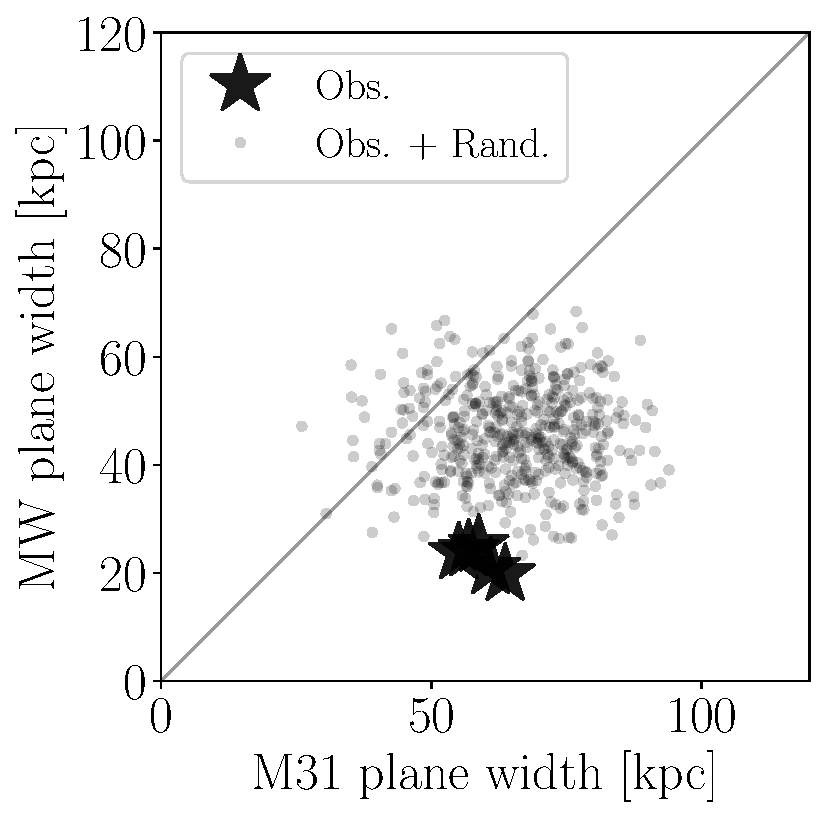
\includegraphics[width=0.30\textwidth]{scatter_random_ranked_width.pdf}
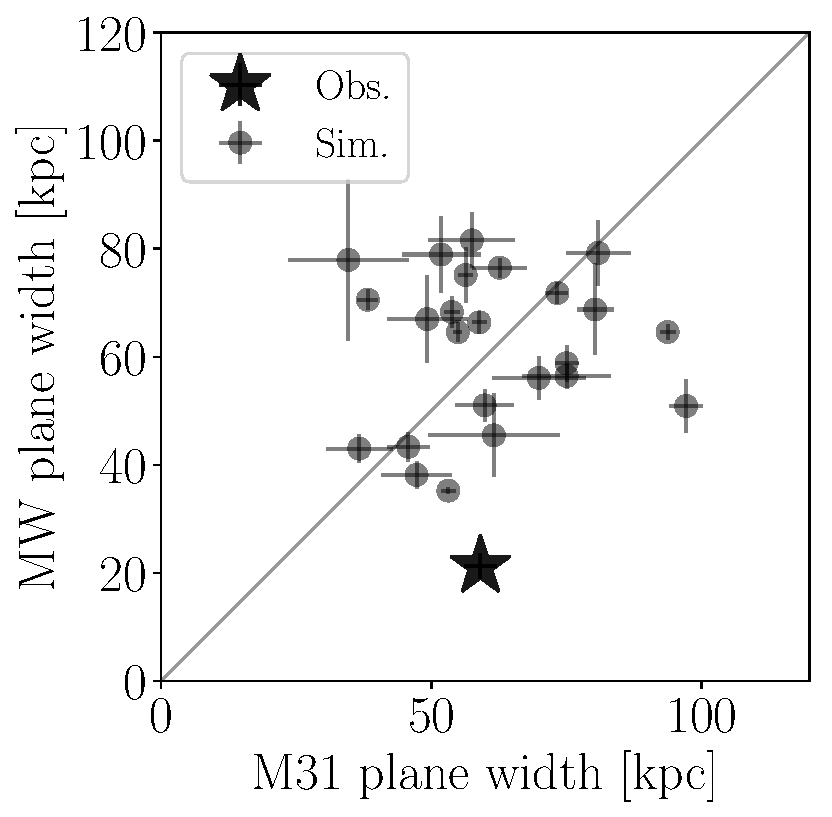
\includegraphics[width=0.30\textwidth]{scatter_ranked_illudm_width.pdf}
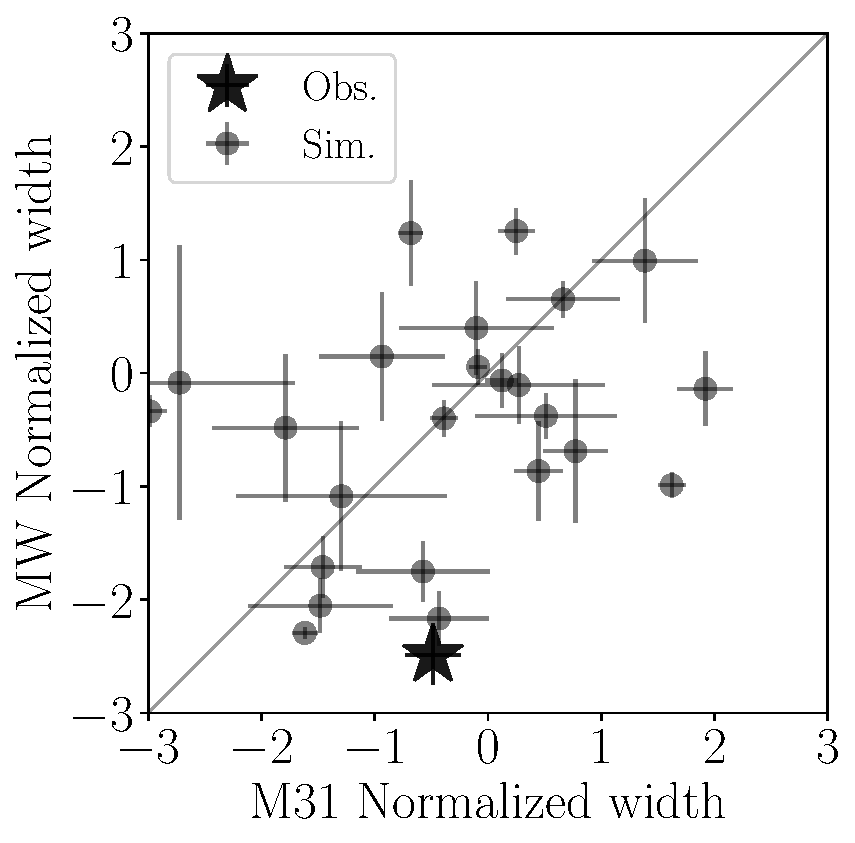
\includegraphics[width=0.30\textwidth]{scatter_norm_ranked_illudm_width.pdf}
\caption{Plane width characterization in observations and
  simulations (Illustris1-Dark in this case.) In all panels the
  horizontal/vertical axis corresponds to the  M31/MW or the
  most/less massive halo in the pair 
  Left. Plane width in physical units comparing the results from observations
(stars) against the result of spherically randomizing the satellite
positions (circles). 
Middle. Average from the observations (star) and the average from each
pair in the simulation (circles).
Right. Same as the middle panel only that this time each point has
been normalized (median substracted and normalized by the standar
deviation) to the results of its randomization. 
The main message of these panels that the MW has a significantly
thiner plane both compared to the result of its own satellite
spherical randomization (left panel) and the expectation from
simulations (middle and right panel).  
This low value is $2\sigma$ away from what is expected in a spherical
distribution. 
In M31 the satellite distribution are in agreement with the
expectations both from an spherical distribution and the results form the
simulations. 
\label{fig:scatter_width}}
\end{figure*}


\begin{figure*}
\centering
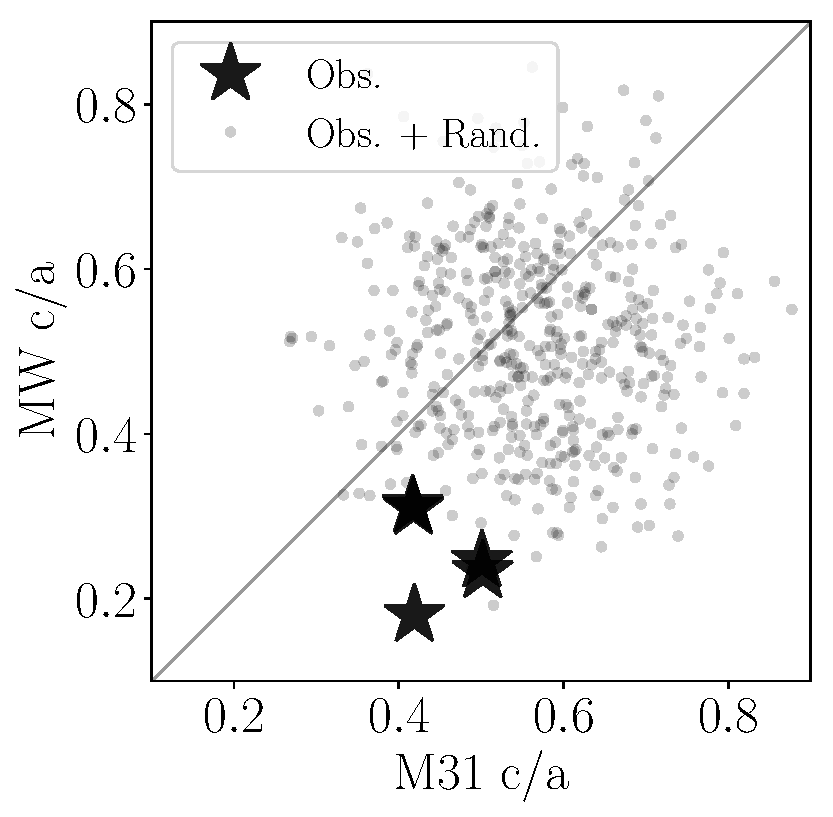
\includegraphics[width=0.30\textwidth]{scatter_random_ranked_ca_ratio.pdf}
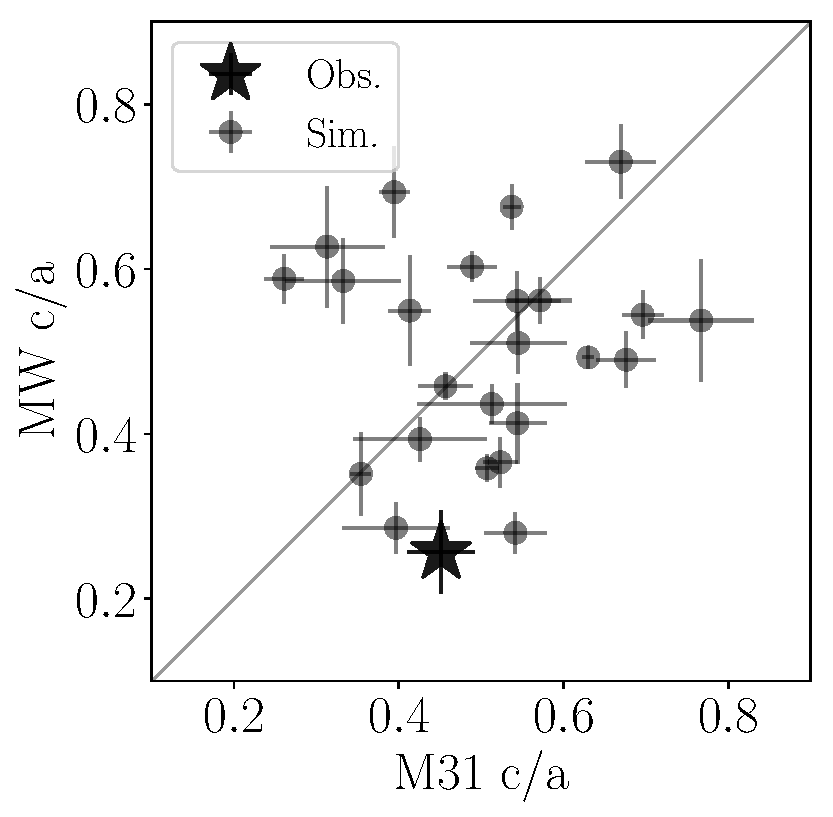
\includegraphics[width=0.30\textwidth]{scatter_ranked_illudm_ca_ratio.pdf}
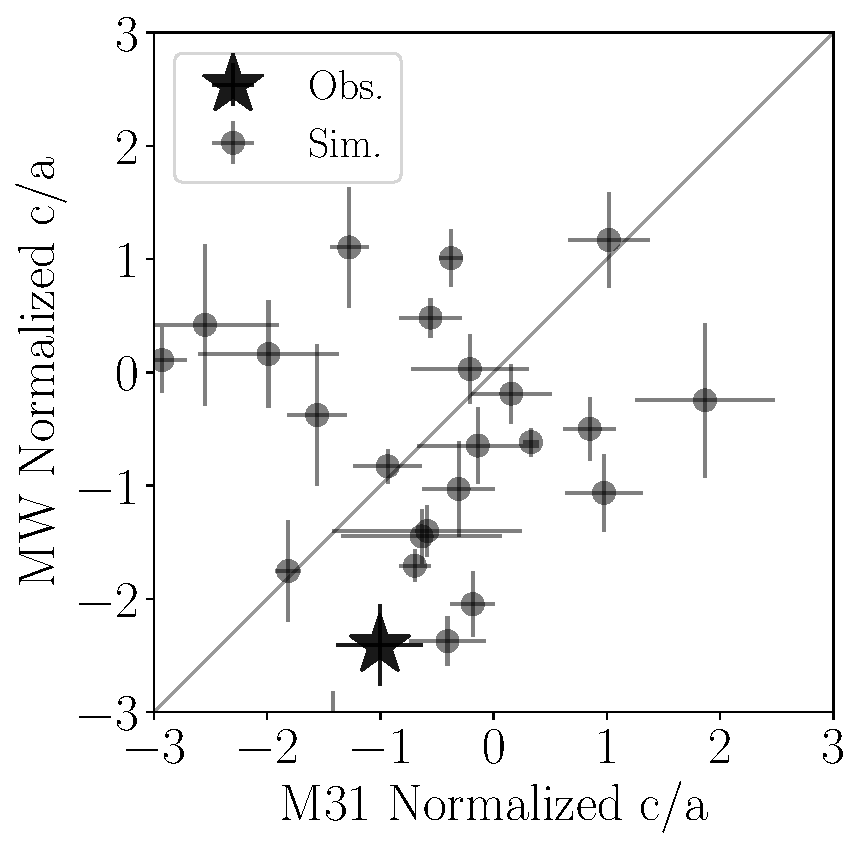
\includegraphics[width=0.30\textwidth]{scatter_norm_ranked_illudm_ca_ratio.pdf}
\caption{Same layout as in Figure \ref{fig:scatter_width}. 
This time for the $c/a$ axis ratio. 
The same message holds in this case; namely, that 
the MW is has a significantly lowwe $c/a$ value than the
expectation from the spherical distribution and the simulations. 
This low value is also $2\sigma$ away from the expactations for an
spherical distribution.
On the other hand, M31 is consistent both with an spherical
distribution and the results from simulations.
\label{fig:scatter_ca_ratio}}
\end{figure*}


\begin{figure*}
\centering
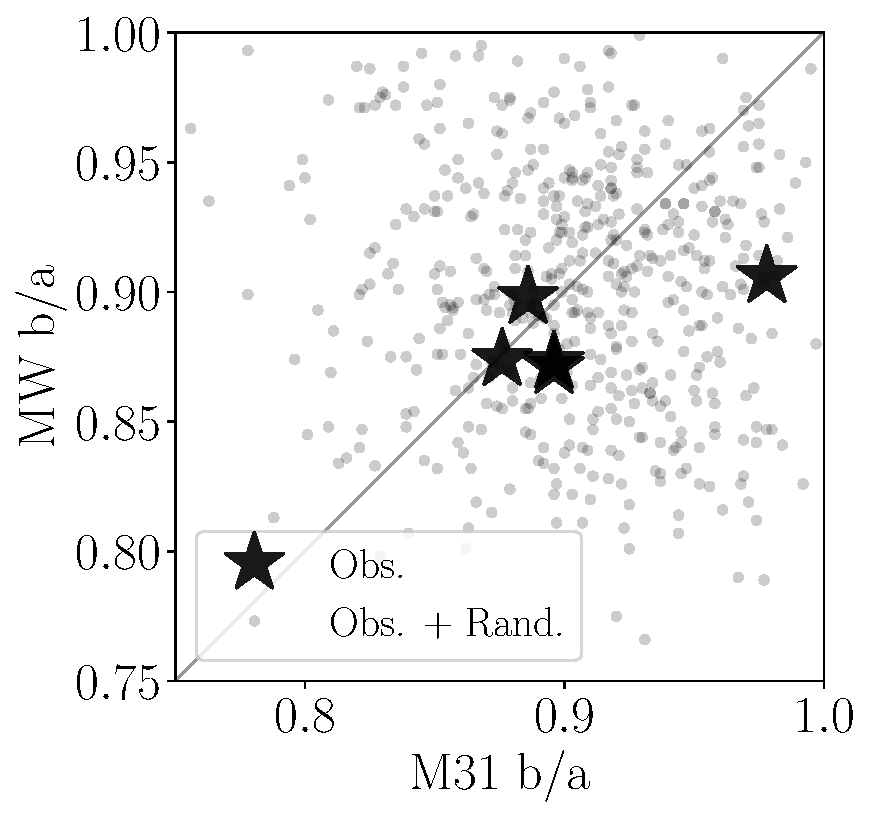
\includegraphics[width=0.30\textwidth]{scatter_random_ranked_ba_ratio.pdf}
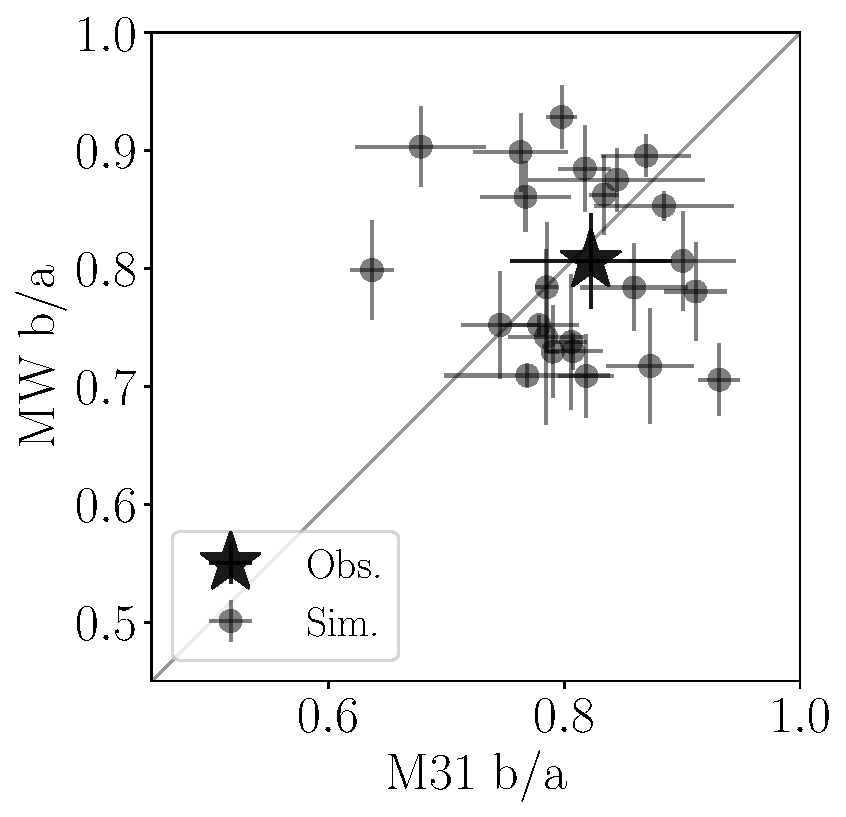
\includegraphics[width=0.30\textwidth]{scatter_ranked_illudm_ba_ratio.pdf}
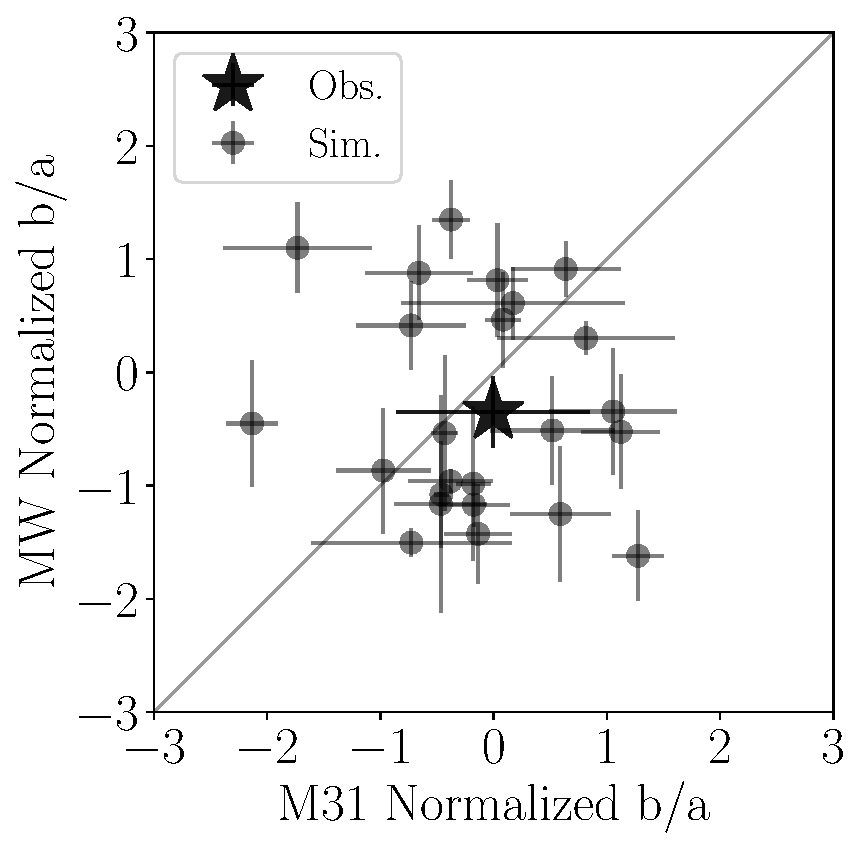
\includegraphics[width=0.30\textwidth]{scatter_norm_ranked_illudm_ba_ratio.pdf}
\caption{Same layout as in Figure \ref{fig:scatter_width}. 
This time for the $b/a$ axis ratio. In this case both the MW and M31
are consistent with the results of a spherical distribution and 
simulations. 
\label{fig:scatter_ba_ratio}}
\end{figure*}


\begin{figure*}
\centering
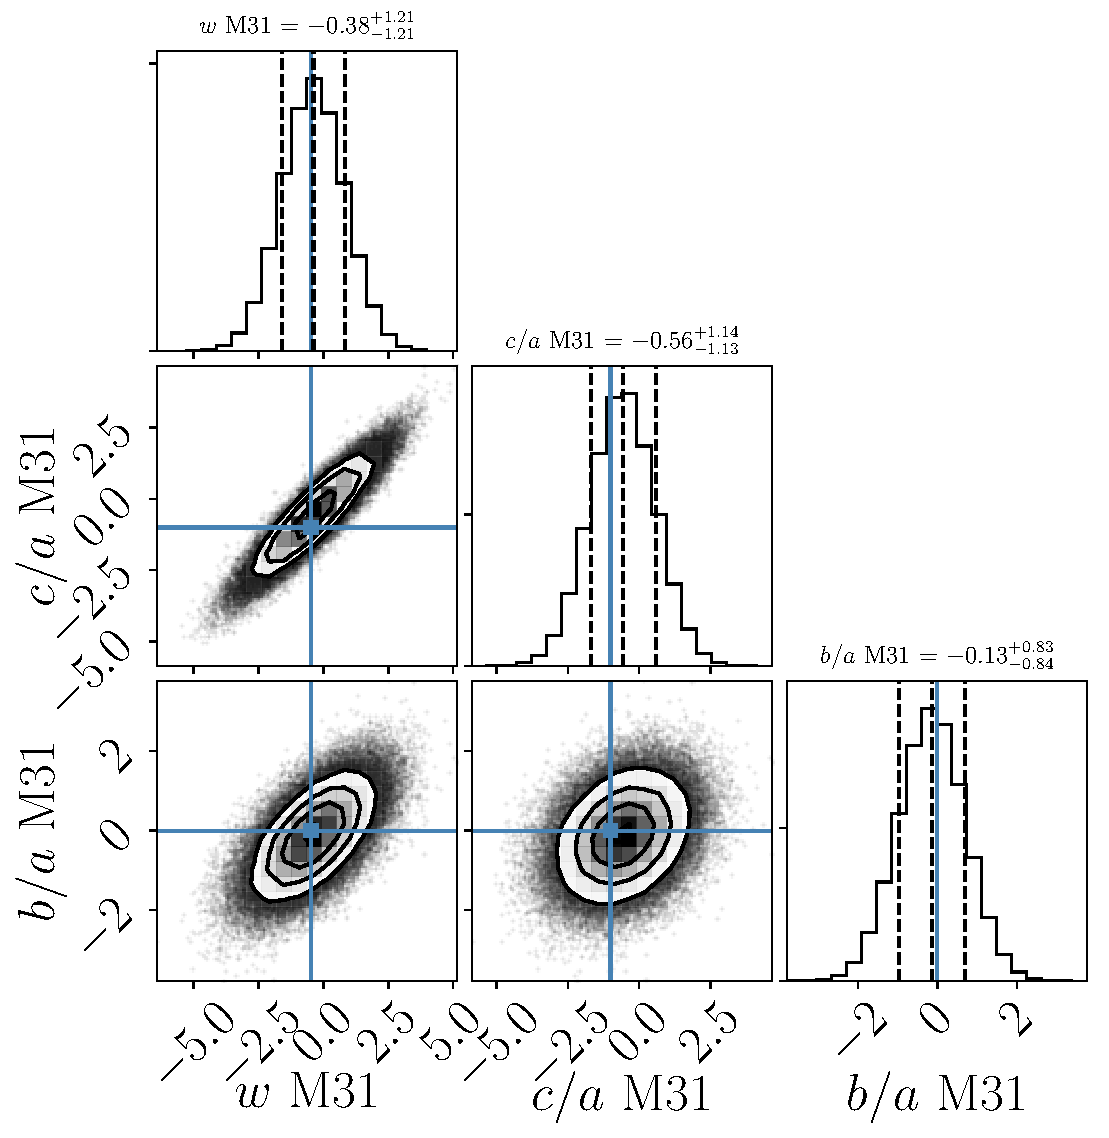
\includegraphics[width=0.45\textwidth]{gaussian_model_illustrisdm_M31.pdf}
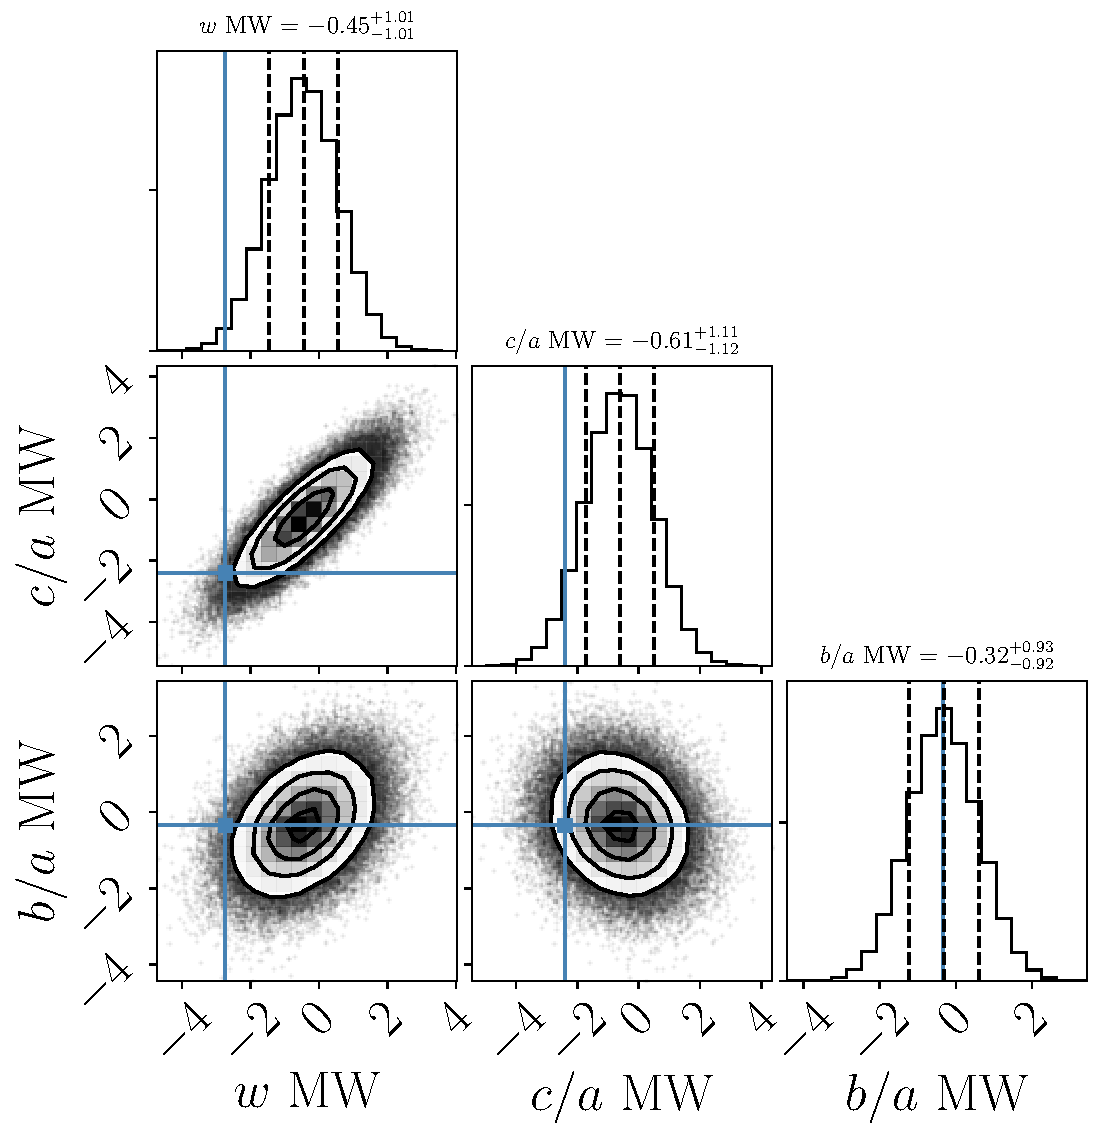
\includegraphics[width=0.45\textwidth]{gaussian_model_illustrisdm_MW.pdf}
\caption{Results from multivariate gaussian model fitted on   the
  normalized values for the plane width $w$, $c/a$ ratio and $b/a$
  ratio from the Illustris1-Dark results.  
  Left/right panel correspond
  to M31/MW.  
  The cross indicates the observed values.
  The contour levels in the 2D histograms correspond to the $1\sigma$,
$2\sigma$ and $3\sigma$ contours in two dimensions.
  The dahsed vertical lines in the histograms along the diagonal
  correspond to the $1\sigma$ boundaries in one dimension.
  The results for the gaussian model are built from $10^6$ point
  realizations in the three-dimensional space spaned by the variables of
  interest for each halo. 
  This plot clearly shows how the M31 results are well within the
  expectations from simulations while the MW has an unusual low value for
  the plane width and the $c/a$ axis ratio.
\label{fig:correlations_illustrisdm}}
\end{figure*}


\section{Results}
\label{sec:results}

Table \ref{table:observations} and Table \ref{table:simulations}
summarize the mean values and uncertainties for the plane $w$, $c/a$
ratio and $b/a$ ratio in the observations and simulations, respectively. 
The uncertainty in the observations is computed over the results with
different number of satellites, while in the simulations it
corresponds to the standard deviation over different halos. 

The observed widths are always smaller than its randomized version.
For M31 there is barely a ratio of $0.92$ between observed and
randomized, while for the MW this factor goes down to less than half
$0.48$. 
The observed $c/a$ ratio follows the same extreme trend for
the MW compared to a M31 distribution closer to spherical, 
The $b/a$ ratio is statisically the same between observations and the
spherical randomization. 


In the following subsections we describe in detail the results on the 
distributions for $w$, $c/a$ and $b/a$. 
The plots in the main body of the paper correspond to the
Illustris1-Dark simulation; the results from the other simulations are
included in the Appendix.

\subsection{Plane Width}

Figure \ref{fig:scatter_width} summarizes the results for the width
measurements.
The left panel compares the results for the MW and M31
observations (stars) against its spherically randomized satellites
(circles). 
The most interesting outcome is that the MW plane width is smaller
than $\approx 98\%$ of the planes computed from the randomized distribution,
while the M31 plane width is only slightly smaller than the average of
the distribution.

The middle panel in Figure \ref{fig:scatter_width} compares the
observational result (star) against the measurements of all pairs from the Illustris1-Dark
simulation (circles).
In this case we have a similar result as before. 
The observed MW width is smaller than all the results in the
simulation, there is not a single halo with similar values.
On the other hand, the results for the M31 are entirely consistend
with observations. Most of the halos in the simulation show a width
value similar to M31. 

The right panel in Figure \ref{fig:scatter_width} shows the result for
the normalized width.  
This panel tells the same story as the middle panel. The M31 values
are typical while the MW is an outlier. 
The added value of the data in this panel is that it is the normalized
which is consistent with normal distributions.
This is the data used to build the mean values vector and covariance
matrix described in Equation 



\begin{figure*}
\centering
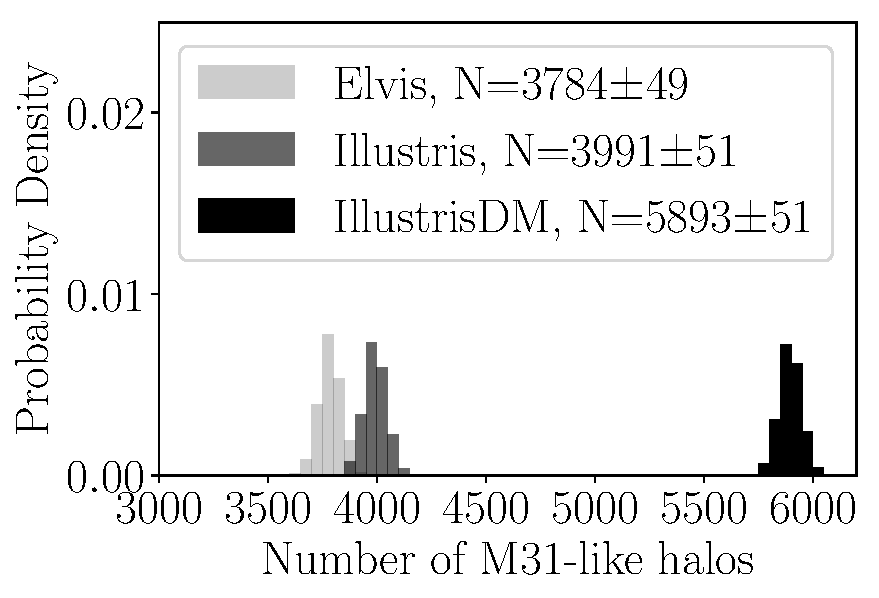
\includegraphics[width=0.47\textwidth]{expected_numbers_n_M31.pdf}
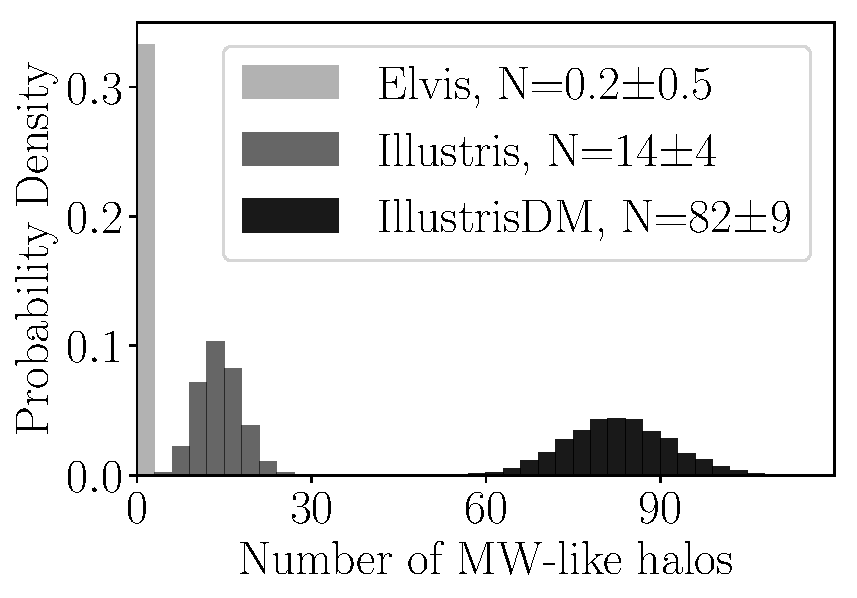
\includegraphics[width=0.47\textwidth]{expected_numbers_n_MW.pdf}
\caption{Probability distribution for the expected number of M31 and
  MW halos  showing the same degree of atipicality as the Local Group if drawn
  from a sample of 10000 isolated pairs. 
  The distributions correspond to results derived from Illustris-DM, Illustris,
  and ELVIS data.
  In the most optimistic case (Illustris-DM), $1\%$ of the pairs have
  two halos with properties similar to the LG. In the case of
  Illustris this percentage drops to $0.1\%$ and $0.01\%$ for ELVIS.
\label{fig:expected_number}}
\end{figure*}

\subsection{$c/a$ axis ratio}

Figure \ref{fig:scatter_ca_ratio} shows the results for the minor to
major axis ratio. 
The layout is the same as in Figure \ref{fig:scatter_width}.
The results for the $c/a$ ratio follow the same trends as for the
width $w$.

The left panel in Figure \ref{fig:scatter_ca_ratio} shows how the MW
the $c/a$ ratio is significantly lower as the measured values for
spherical distributions, it is smaller than $\approx 98\%$ of the
randomized distributions.   
On the other hand the ratio for M31 is lower than the mean of the
spherical values but still well within its variance.

The middle panel in the same Figure shows the LG compared against the
results in the simulations. 
In this case we find a similar trend as before. 
The MW is atypical and M31 is within the variance from the simulation data.
This time, however, there are two MW-like halos out of the total
of 24 that show an $c/a$ as small as the MW.

The right panel shows the normalized results. 
The MW shows a low $c/a$ ration close to between two and three
standard deviations away from the mean value of the spherical
distribution; this contrasts the results for M31 which are close to
$1$ standard deviation away. 


\subsection{$b/a$ axis ratio}

Figure \ref{fig:scatter_ba_ratio} shows the results for the minor to
major axis ratio with the same layout as Figure \ref{fig_scatter_ca_ratio}
In all cases of comparison (against randomized distribution
and simulations  the results for both the MW and M31 are typical. 


\subsection{Fit to a Multivariate Gaussian Distributions}



Figure \ref{fig:correlations_illustrisdm} illustrates the results from
 compute the covariance matrix and mean vector in
 Eq.\ref{eq:multivariate} from the normalized quantities computed from
 the Illlustris1-Dark simulation.
The distributions in the Figure are computed from $10^6$ with the multivariate
gaussian. 
Similar plots for Illustris1 and ELVIS are in the Appendix.
The values for all the covariance matrices and mean vectors for all
the simulations are listed in the Appendix.

This results nicely summarizes the results we had in the previous
sections. 
The left triangular plot shows how M31 falls into the middle of all 2D
distributions always close to the peak and within the $1-\sigma$
range. 
The right plot clearly places the MW observations outside the
$3\sigma$ range in the joint distributions that involve the width
$w$. 

In both cases the strongest positive correlation is present for the
width and the $c/a$ axis ratio. A weaker but still positive
correlation is present for the width and the $b/a$ axis ratio.



\subsection{Number of Expected LG Systems}

We us the fits to the multivariate gaussian distributions to
compute the expected number of pairs with characteristics similar to
the LG.
To do this we generate $10^3$ samples, each sample contains $10^4$
pairs, where each pair member is drawn from the corresponding
multivariate gaussian distributions.  

We consider that a sampled system is similar to the M31/MW galaxy if the
distance of each of its characteristics ($w$, $c/a$, $b/a$) to the
sample mean is equal or larger than the distance of the observational
values to the sample mean.   
That is, we perform a double-tailed test using the observational
values as a threshold. 

Figure \ref{fig:expected_number} summarizes the results from this
experiment. 
The left panel shows the probability density for the number of M31
systems in a parent sampe of $10^4$ pairs, the right panel shows the
results for the MW.
For M31, between $37\%$ to $58\%$ of the pairs have a satellite
distribution as aspherical as M31 in observations; this fraction drops
dramatically for the MW where only $0.03\% to 2\%$ of the satellites
are expected to have extreme aspherical distributions as the MW.

Considering the joint distribution of M31 and MW we find that at most
$1\%$ of the pairs are expected to be similar to the LG.
In a three dimensional gaussian distribution, having a $1\sigma$,
$2\sigma$ and $3\sigma$ interval corresponds to have respectively $19 \%$, $73 \%$ and
$97 \%$ of the total of points in the distribution.
With this result in mind the $LG$ has the same degree of atipicality
as an $3\sigma$ outlier. 
% FUNDAMENTALS OF MULTIVARIATE STATISTICS, for Imaging and optics,
% Bajorski.
%In [150]: stats.chi2.cdf(l**2,3)
%Out[150]: array([ 0.19874804,  0.73853587,  0.97070911])

Among the three simulations, the results infered from ELVIS data show
the lowest fraction of M31 and MW systems; for Illustris1-Dark we have
the highest fraction of M31/MW systems. The results from Illustris1
are in between these two, actually closer to ELVIS.



\section{Conclusions}

In this paper we develop and demostrate a method to quantify the
asphericity of the satellite distribution in the Local Group.
We build up on the suggestions made in \cite{XX}.
We do not look for planes or coherent kinematical structures in the
interest of keeping the method straightforward and robust.

The method uses as a reference point the spherically randomized data
of the system under study.
We first measure the width and axis ratios for the satellite
distribution of interest. 
Then, we measure the same quantities for spherically
randomized data. 
Finally, renormalize the initial results to the mean value and
standard deviation from the randomized samples.  

The normalized quantities for different systems are well reproduced by
a multivariate gaussian distribution. 
We fit the parameters of this gaussian to the results from 
LG samples coming from three different simulations
to finally compare the observational results against the distributions
derived from the simulations.


We find that in the best case (Illustris1-DarkMatter) the deviation
from aesphericity in the observed LG is only  expected in $3\pm2$
pairs out of a sample of $10^4$ isolated pairs. This places the LG as
a $3\sigma$ outlier.   
The weight to explain this atypical result is not distributed equally
between the MW and M31. 
While M31 presents a fully typical asphericity in the expectations
from LCDM, the MW shows aspherical deviations in plane width and the
major-to-minor axis ratio highly atypical in the 
framework of LCDM. 
We estimate that with the M31 between $37\%$ and $58\%$ of the pairs
pairs show normalized characteristics larger than M31, while
this fraction drops to less than $1\%$ for the MW.
These fractions are robust to changes in the numerical simulations and to
the criteria used to define the pairs.


The highly aspherical distribution of the brightest MW satellites is
in stark contrast to the more spherical M31 distribution.
Furthermore, the atipicallity of the MW distribution in the LCDM
context adds up to the also atypical presence of two bright satellite
galaxies.


The focus of our approach is building explicit probability
distributions for the observables of interest, instead of trying to
find simulated objects that fullfil different observational criteria. 
This approach is particularly useful in the case of atypical
observables. 
Building the probability distribution allows for an atypicallity
quantification without needing to build explicit samples of objects
that are already scarce and difficult to find in simulations.

An extension of this framework to outliers in higher order deviations
(i.e. a \emph{subset} of satellites that are in a plane or
coherent \emph{velocity} strictures) should also be possible, similar
to the work presented by XX on the satellite velocity anisotropy.

From the results we derive in this paper we also estimate that a
cosmological volume of at least $( XX )^3$ is required to find a halo pair
that shows similar asphericity characteristics as the LG. 
This atypical satellite distribution should be seen as an opportunity
to constrain in high detail the initial conditions and environment
that allowed such a pattern to emerge. 



\bibliographystyle{mnras}
\bibliography{Dwarfs}

%% Alignments between galaxies, satellite systems and haloes
%% https://arxiv.org/pdf/1605.01728.pdf

%M31 mass
%% https://arxiv.org/abs/1410.0017

%MW mass
%https://arxiv.org/abs/1407.1078
\newpage

\appendix

\section{Physical Characteristics of the Isolated Pairs samples}

\begin{figure*}
\centering
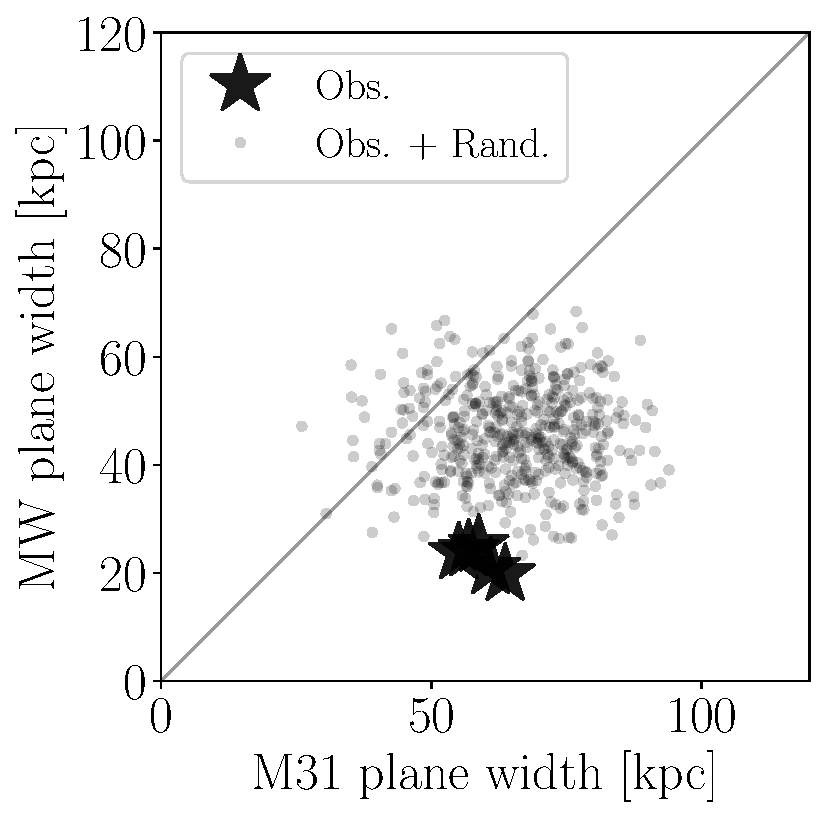
\includegraphics[width=0.30\textwidth]{scatter_random_ranked_width.pdf}
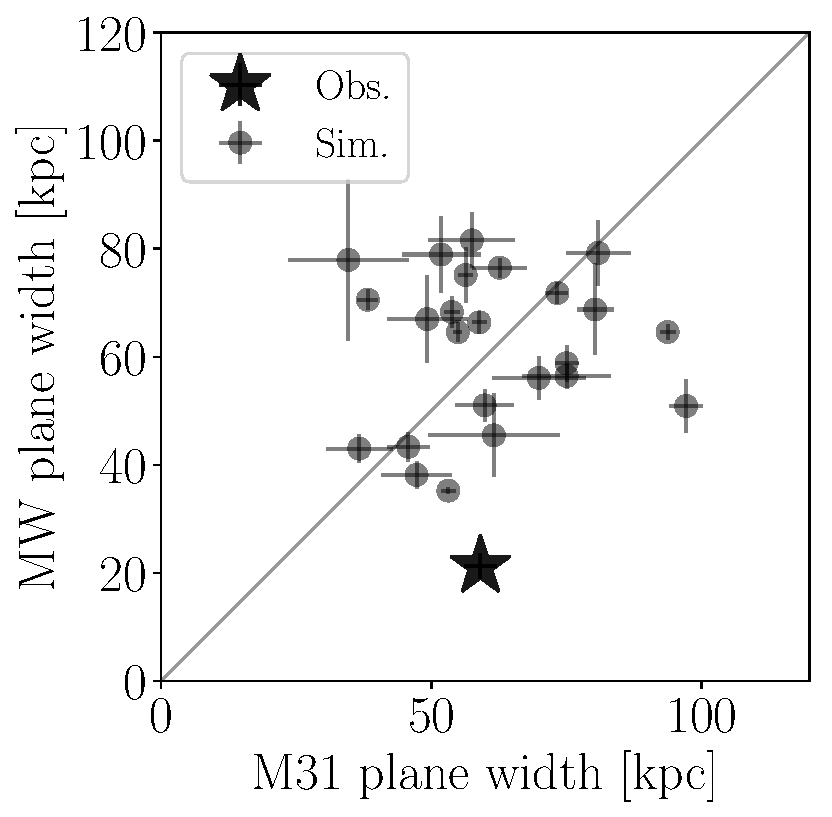
\includegraphics[width=0.30\textwidth]{scatter_ranked_illudm_width.pdf}
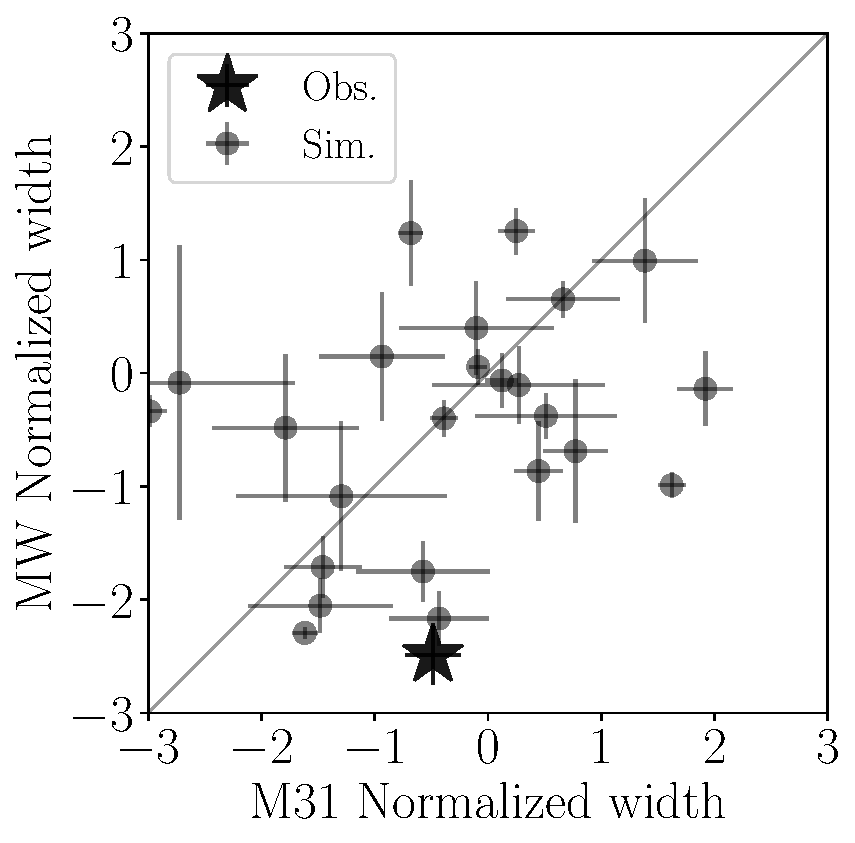
\includegraphics[width=0.30\textwidth]{scatter_norm_ranked_illudm_width.pdf}
\caption{
\label{fig:physical}}
\end{figure*}

\section{Results from ELVIS and Illustris1}
\begin{figure*}
\centering
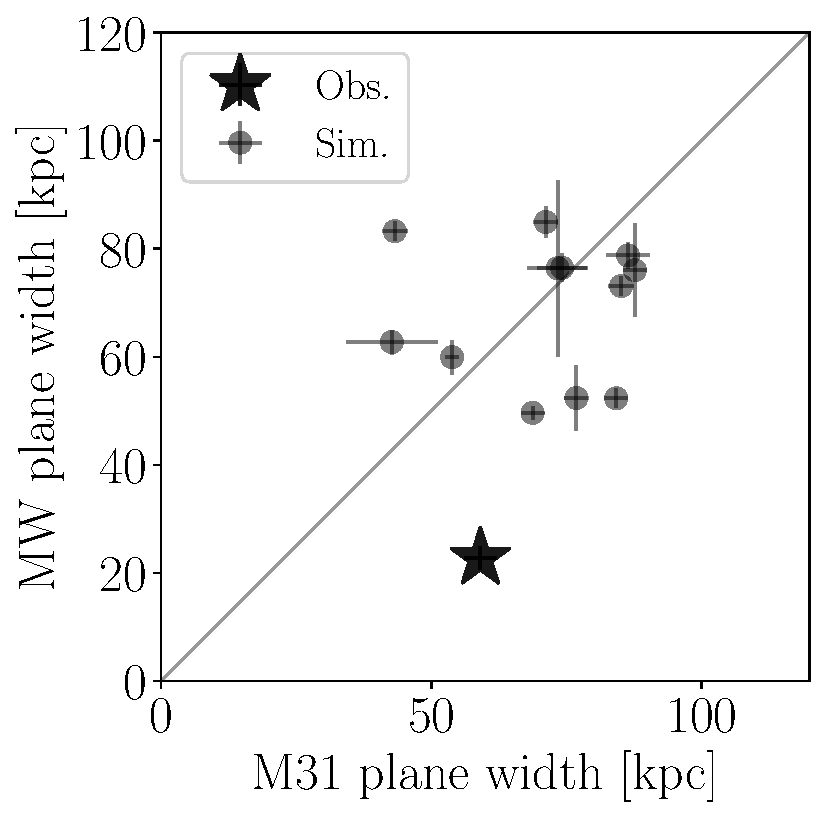
\includegraphics[width=0.28\textwidth]{scatter_ranked_elvis_width.pdf}
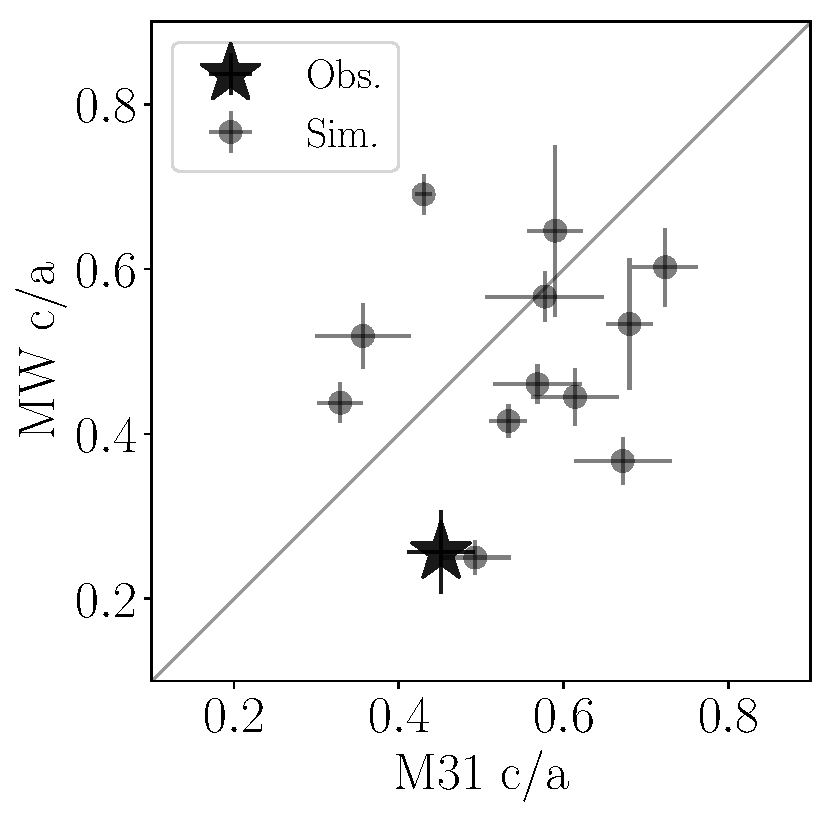
\includegraphics[width=0.28\textwidth]{scatter_ranked_elvis_ca_ratio.pdf}
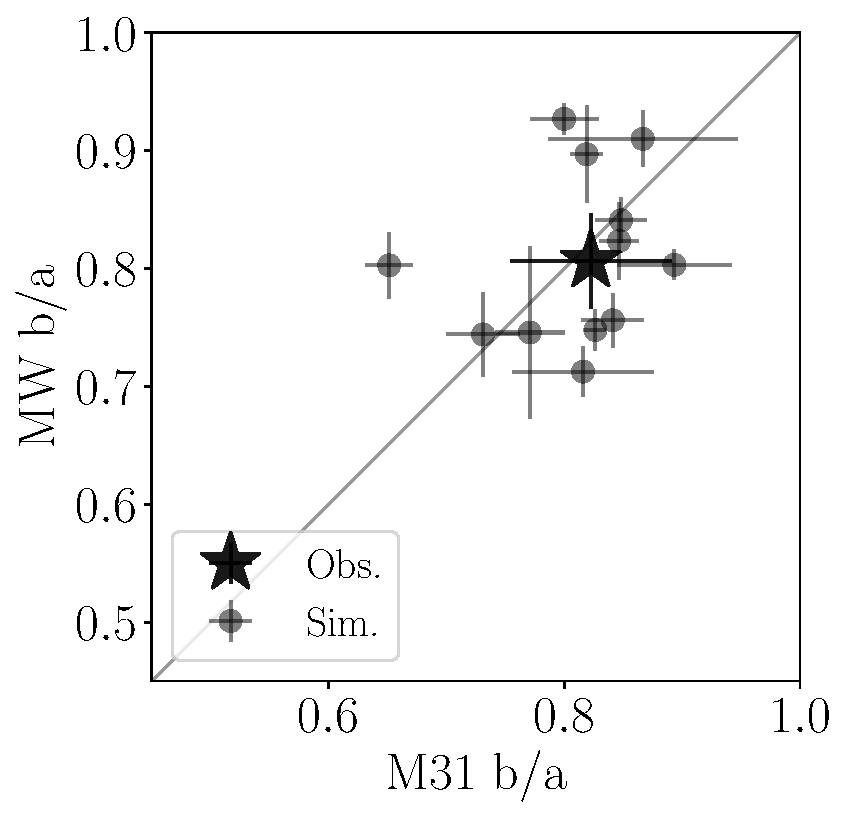
\includegraphics[width=0.28\textwidth]{scatter_ranked_elvis_ba_ratio.pdf}
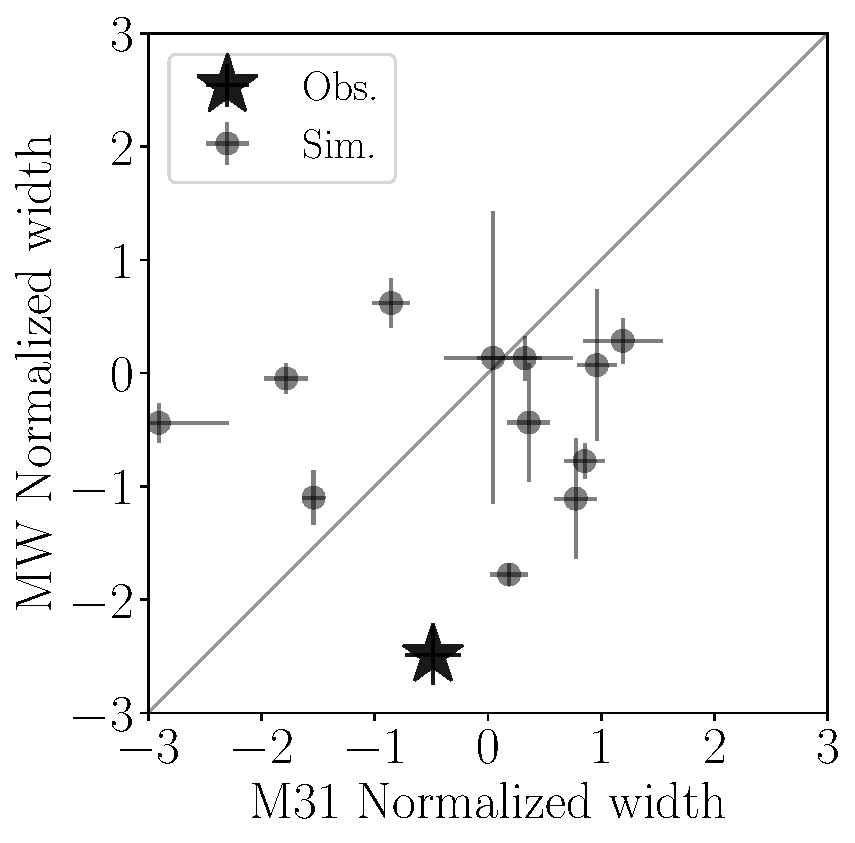
\includegraphics[width=0.28\textwidth]{scatter_norm_ranked_elvis_width.pdf}
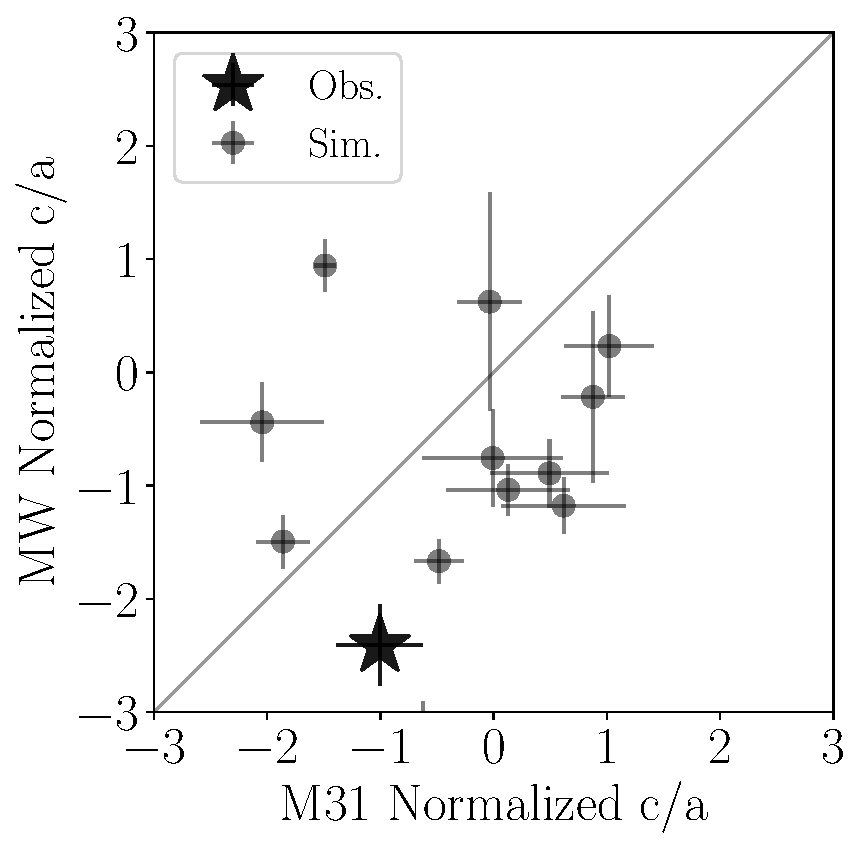
\includegraphics[width=0.28\textwidth]{scatter_norm_ranked_elvis_ca_ratio.pdf}
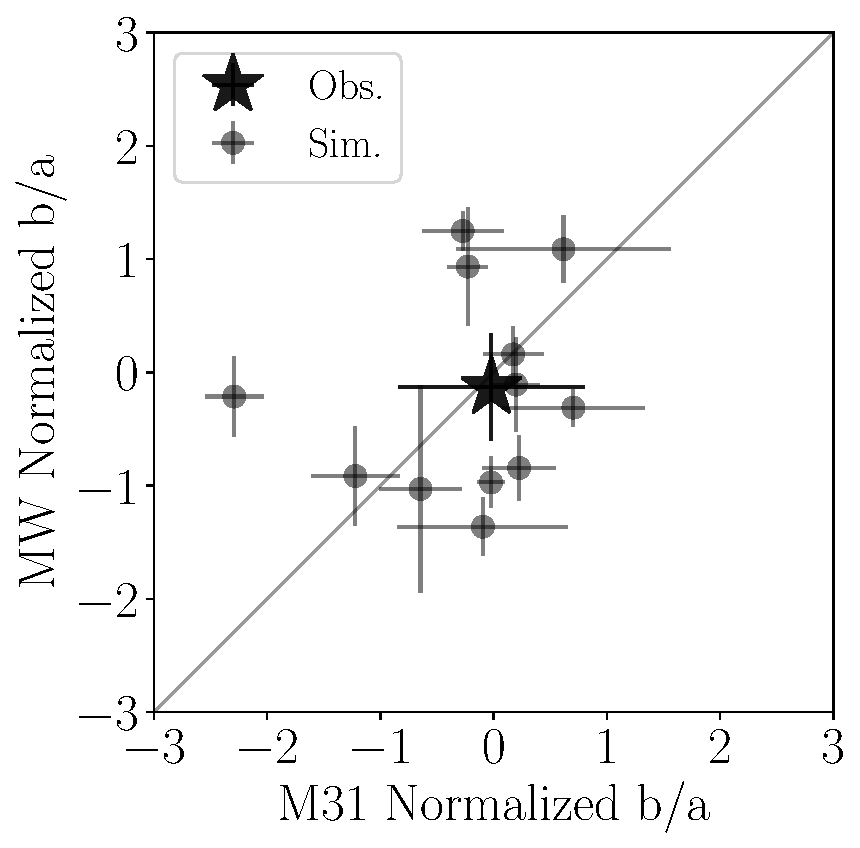
\includegraphics[width=0.28\textwidth]{scatter_norm_ranked_elvis_ba_ratio.pdf}
\caption{ELVIs results for the quantities presented for the Illustris1-Dark
  simulation in Figures  \ref{fig:scatter_width},
  \ref{fig:scatter_ca_ratio}, \ref{fig:scatter_ba_ratio}.
Upper row corresponds to the raw values from observations and
simulated pairs, while the second row normalizes the same values to
the mean and standard deviation on its spherically randomized
counterparts. 
\label{fig:scatter_elvis}}
\end{figure*}

\begin{figure*}
\centering
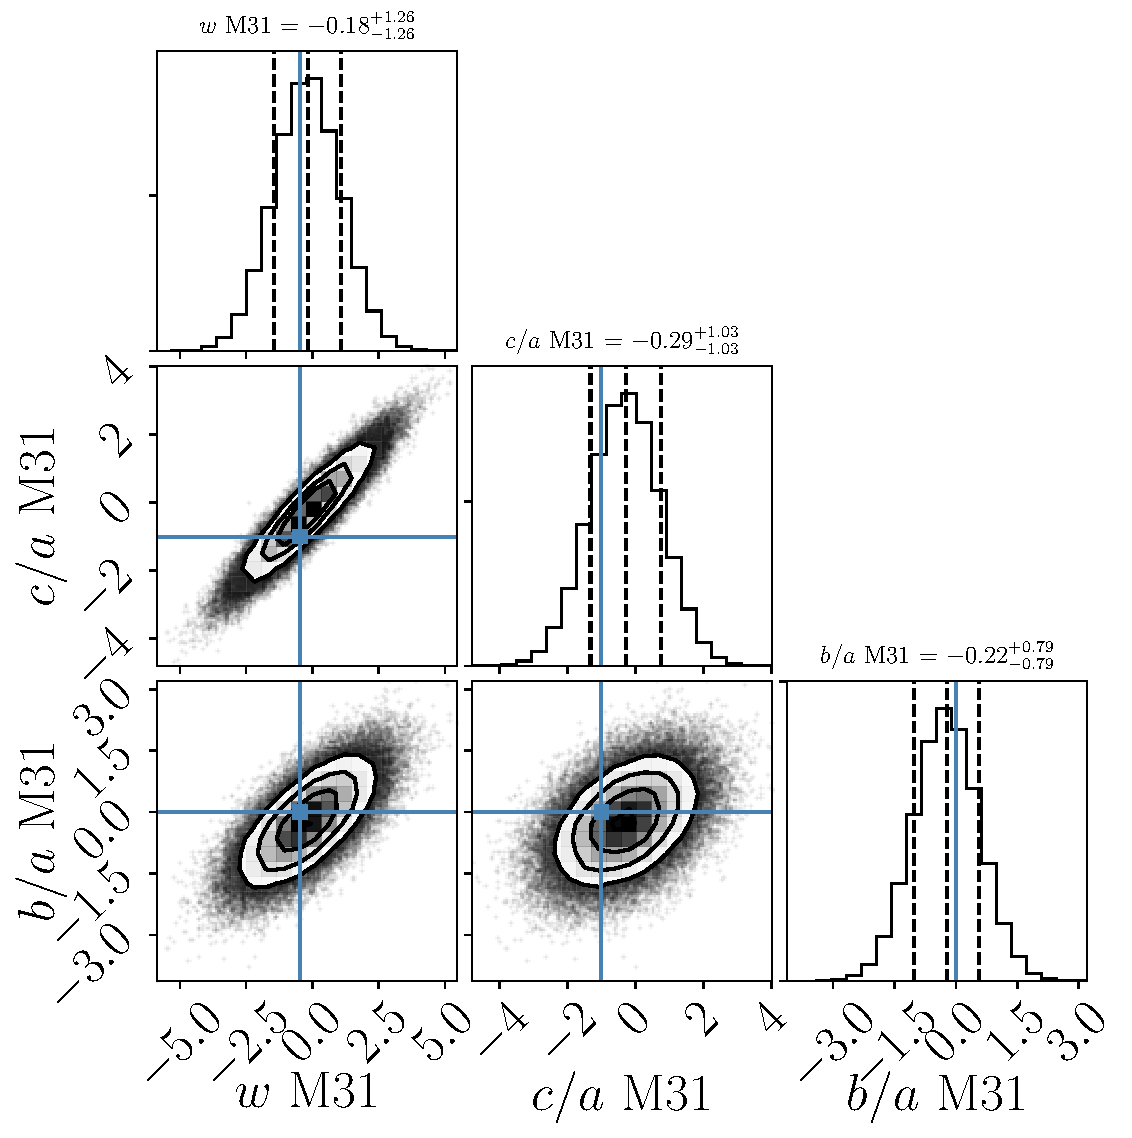
\includegraphics[width=0.45\textwidth]{gaussian_model_elvis_M31.pdf}
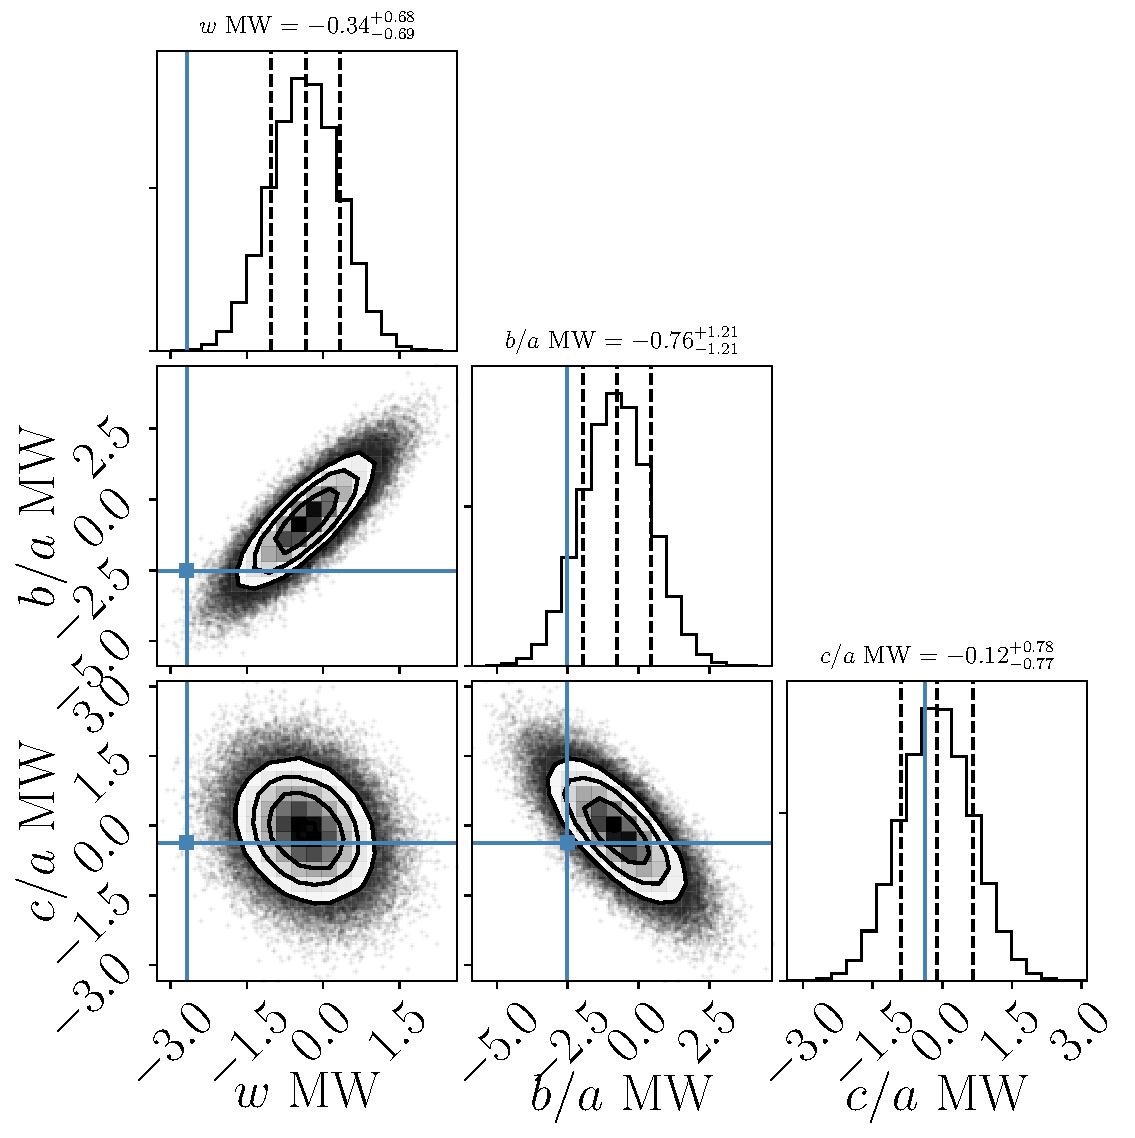
\includegraphics[width=0.45\textwidth]{gaussian_model_elvis_MW.pdf}
\caption{
Same layout as Figure \ref{fig:correlations_illustrisdm}, this time
computed from the ELVIS data.
\label{fig:correlations_elvis}}
\end{figure*}


\begin{figure*}
\centering
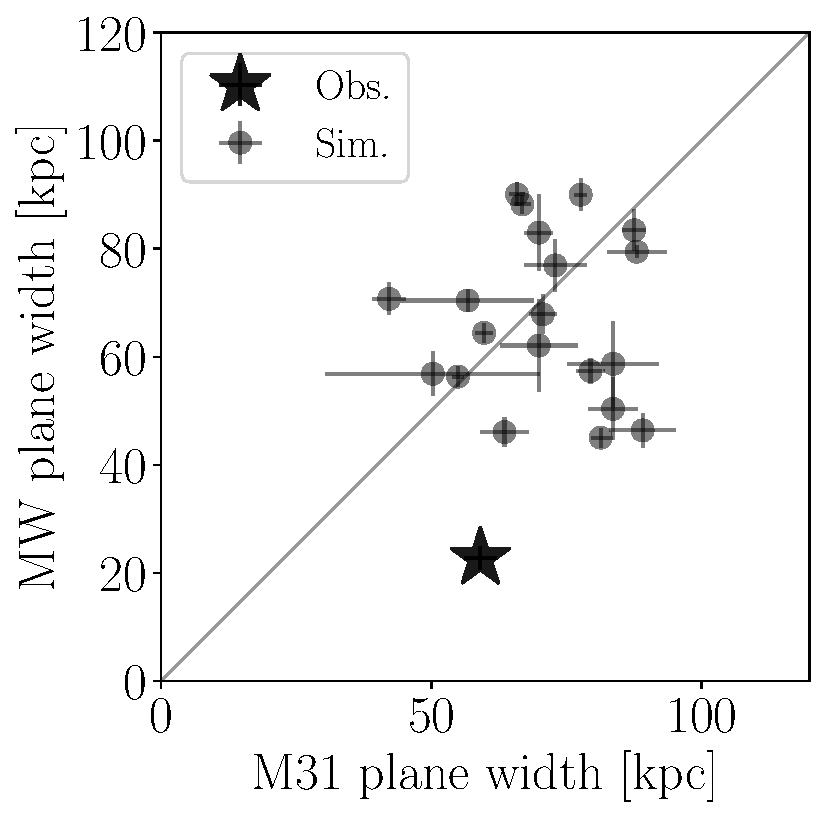
\includegraphics[width=0.28\textwidth]{scatter_ranked_width.pdf}
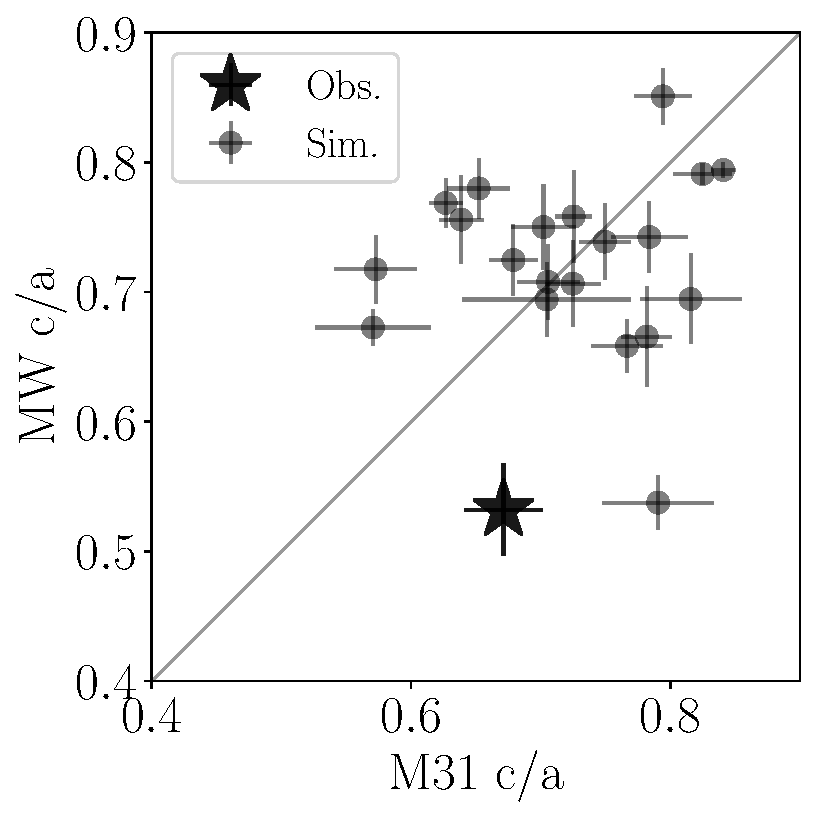
\includegraphics[width=0.28\textwidth]{scatter_ranked_ca_ratio.pdf}
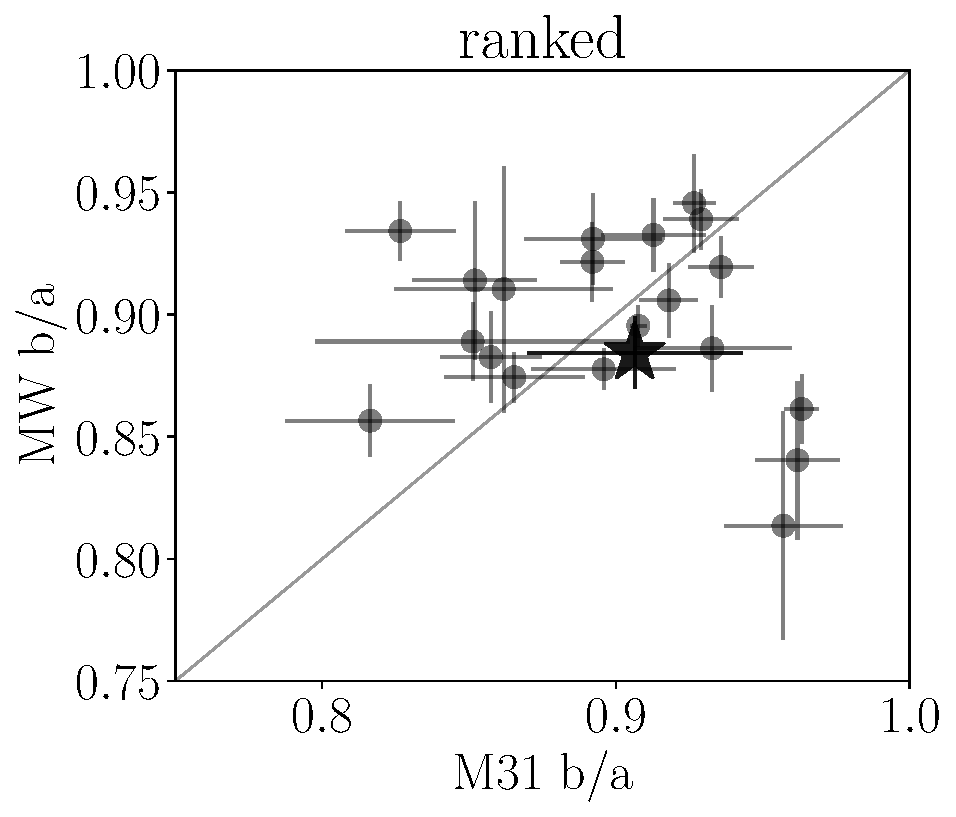
\includegraphics[width=0.28\textwidth]{scatter_ranked_ba_ratio.pdf}
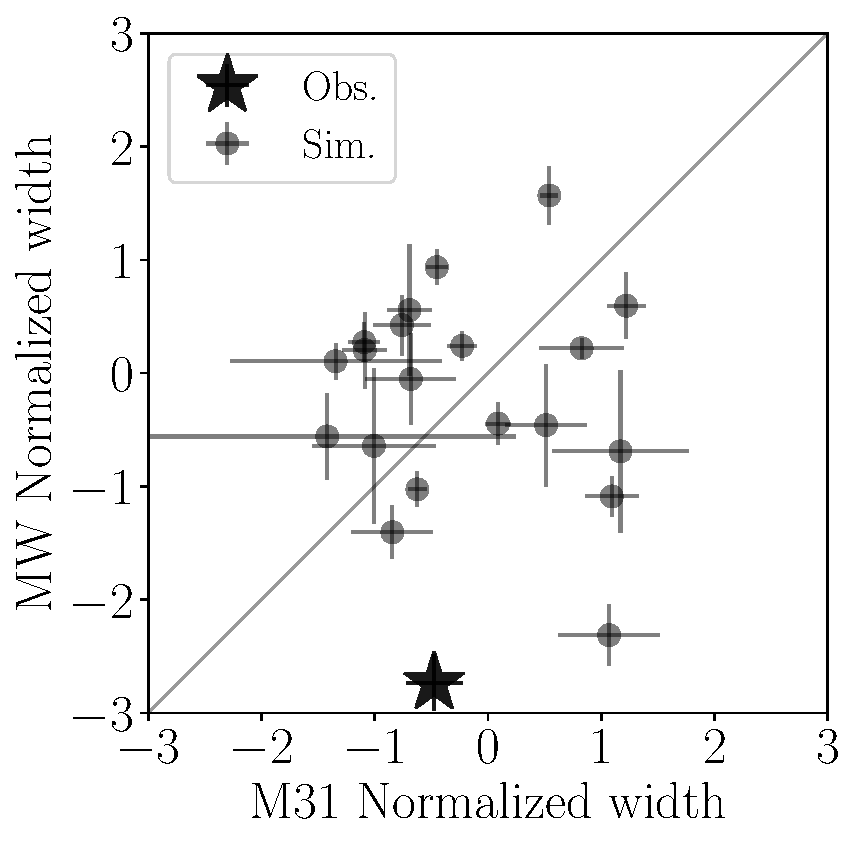
\includegraphics[width=0.28\textwidth]{scatter_norm_ranked_width.pdf}
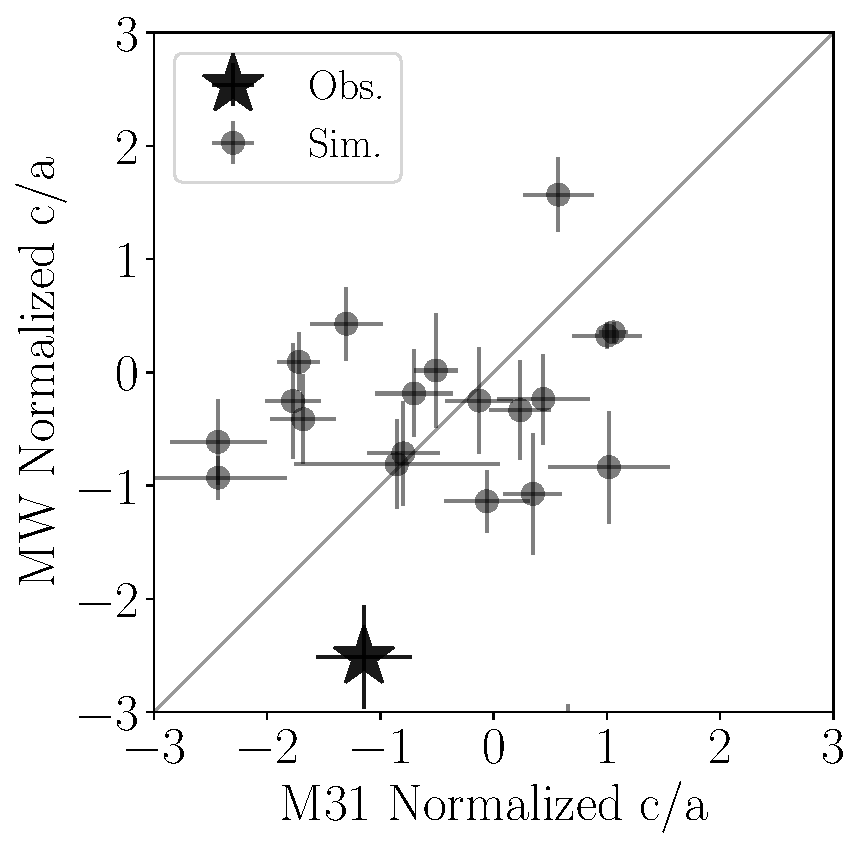
\includegraphics[width=0.28\textwidth]{scatter_norm_ranked_ca_ratio.pdf}
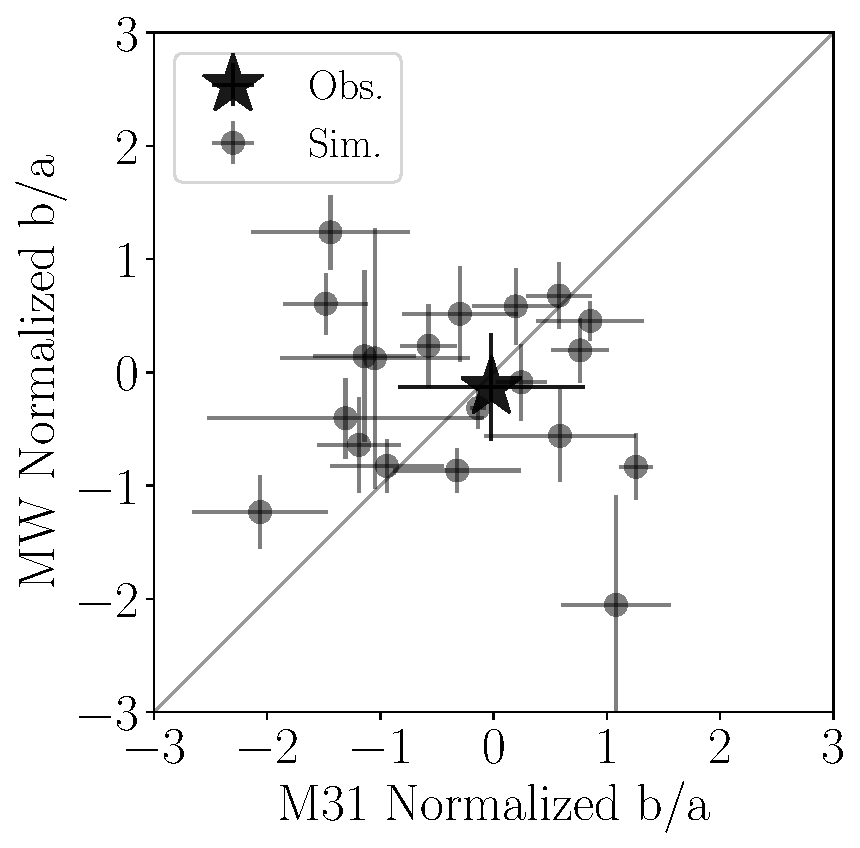
\includegraphics[width=0.28\textwidth]{scatter_norm_ranked_ba_ratio.pdf}
\caption{Same layout as Figure \ref{fig:scatter_elvis}, this time
  computed from the Illustris1 data.
\label{fig:scatter_illustris}}
\end{figure*}


\begin{figure*}
\centering
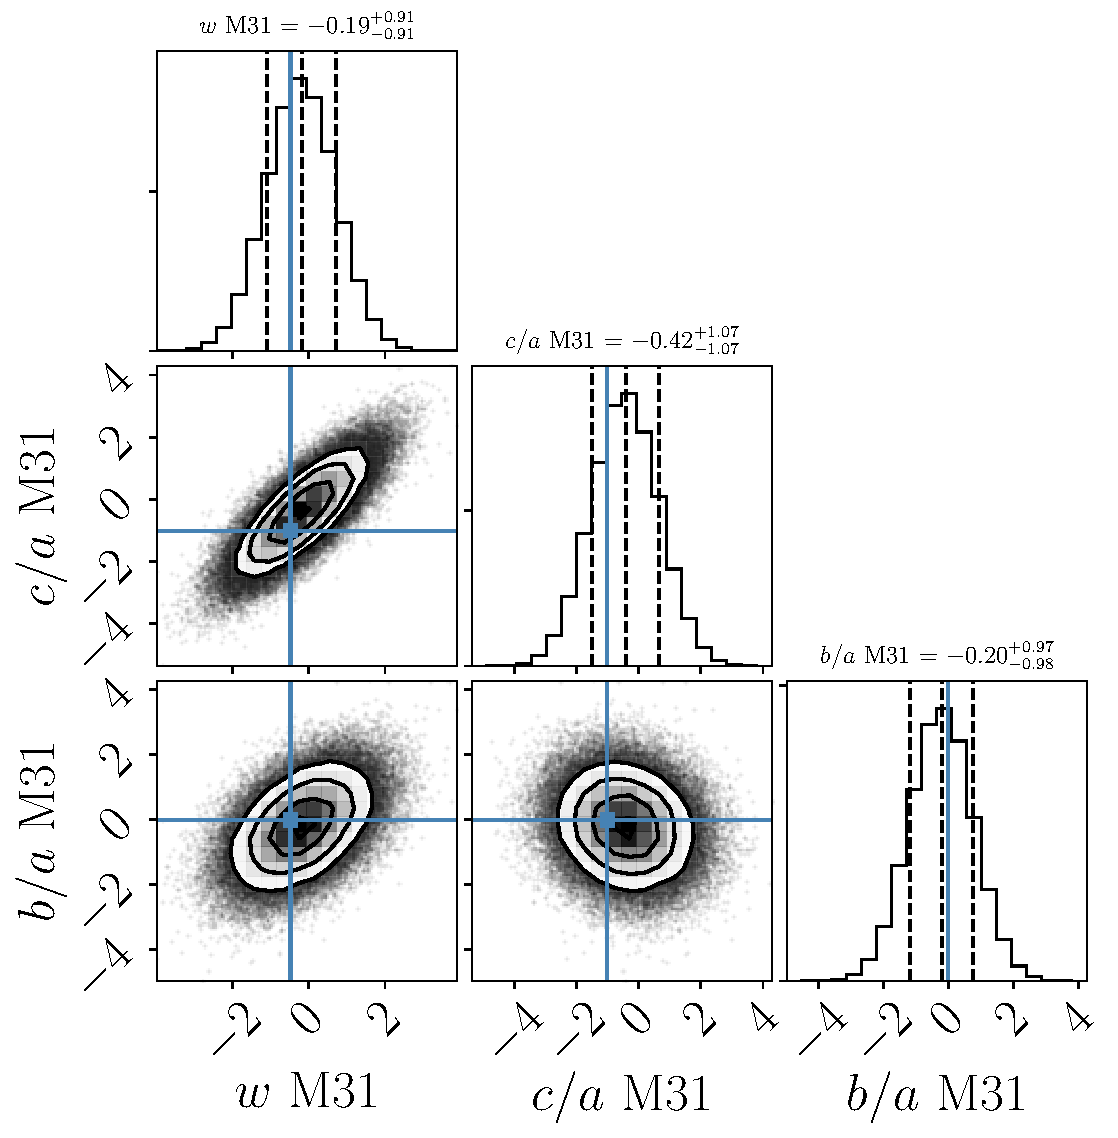
\includegraphics[width=0.45\textwidth]{gaussian_model_illustris_M31.pdf}
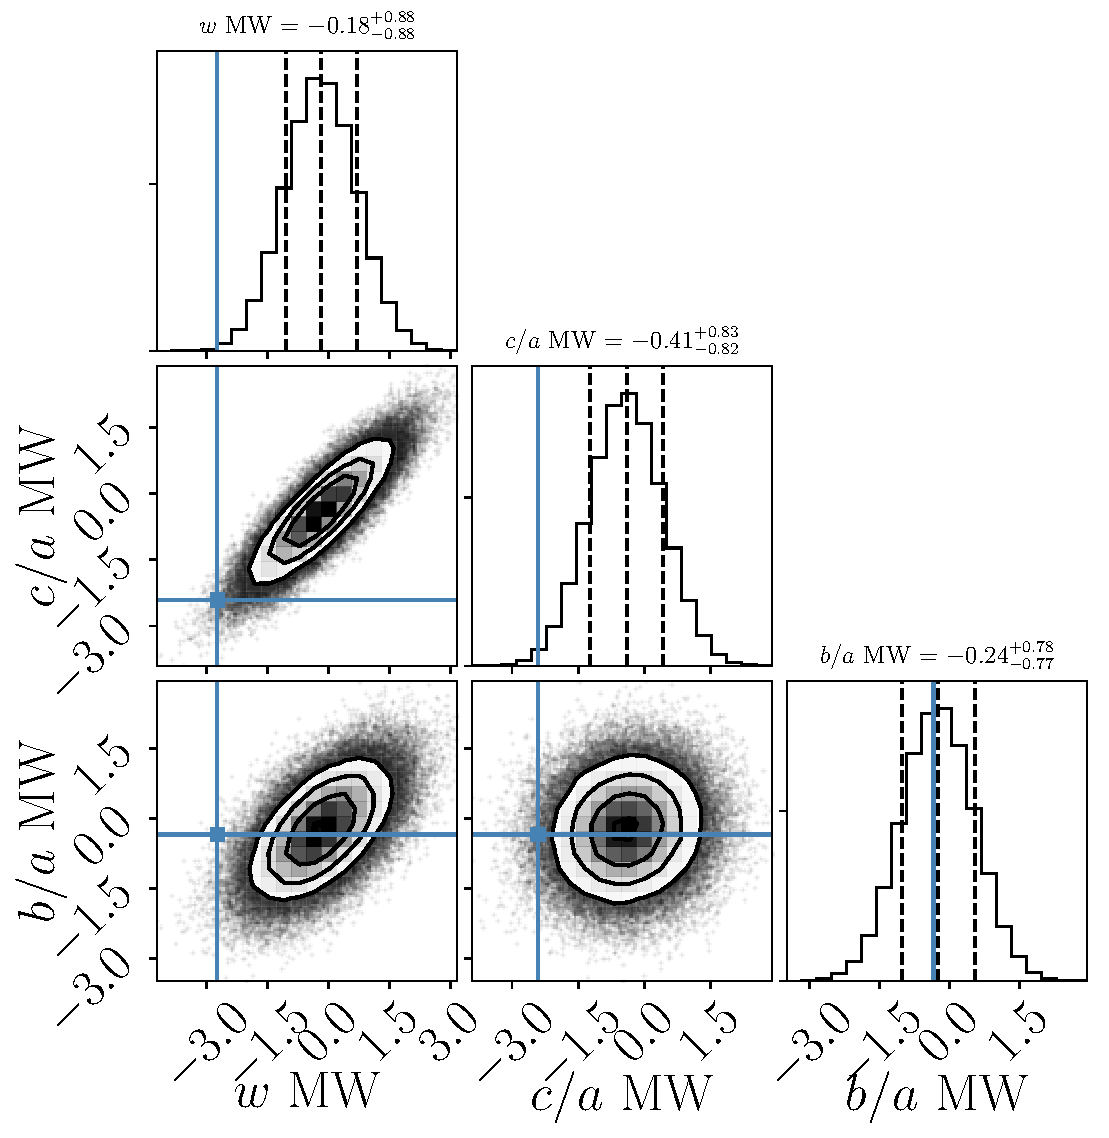
\includegraphics[width=0.45\textwidth]{gaussian_model_illustris_MW.pdf}
\caption{
Same layout as Figure \ref{fig:correlations_illustrisdm}, this time
computed from the Illustris1 data.
\label{fig:correlations_illustris}}
\end{figure*}



\section{Covariance Matrices and Mean value vectors}
Illustris M31

Covariance
\begin{verbatim}
[[ 0.83+/-0.03  0.78+/-0.04  0.41+/-0.04]
 [ 0.78+/-0.04  1.16+/-0.05 -0.15+/-0.05]
 [ 0.41+/-0.04 -0.15+/-0.05  0.96+/-0.04]]
\end{verbatim}

Mean

\begin{verbatim}
[-0.18+/-0.04 -0.41+/-0.05  -0.20+/-0.05]
\end{verbatim}

Illustris MW
\begin{verbatim}
[[ 0.78+/-0.06  0.63+/-0.07  0.40+/-0.03]
 [ 0.63+/-0.07  0.69+/-0.08   0.06+/-0.02]
 [ 0.40+/-0.03  0.06+/-0.02   0.61+/-0.04]]
\end{verbatim} 

Mean
\begin{verbatim}
[-0.17+/-0.04 -0.40+/-0.04 -0.23+/-0.04]
\end{verbatim}



IllustrisDM M31

Covariance
\begin{verbatim}
[[ 1.50+/-0.08  1.27+/-0.08  0.64+/-0.04]
 [ 1.27+/-0.08  1.31+/-0.08  0.28+/-0.04]
 [ 0.64+/-0.04  0.28+/-0.04  0.70+/-0.04]]
\end{verbatim}

Mean
\begin{verbatim}
[-0.37+/-0.05 -0.55+/-0.05  -0.13+/-0.03]
\end{verbatim}

IllustrisDM M31

Covariance
\begin{verbatim}
[[ 1.03+/-0.05  0.94+/-0.05  0.36+/-0.03 ]
 [ 0.94+/-0.05  1.24+/-0.07 -0.18+/-0.04]
 [ 0.36+/-0.03  -0.18+/-0.04  0.86+/0.03]]
\end{verbatim}

Mean
\begin{verbatim}
[-0.45+/-0.04 -0.61+/-0.05 -0.31+/-0.04]
\end{verbatim}

ELVIS M31

Covariance
\begin{verbatim}
[[ 1.60+/-0.19  1.22+/-0.14  0.70+/-0.09]
 [ 1.22+/-0.14  1.08+/-0.10  0.35+/-0.05]
 [ 0.70+/-0.09  0.35+/-0.05  0.63+/-0.10]]
\end{verbatim}

Mean
\begin{verbatim}
[-0.18+/-0.08 -0.28+/-0.07 -0.22+/-0.05]
\end{verbatim}

ELVIS MW
Covariance
\begin{verbatim}
[[ 0.45+/-0.04    0.61+/-0.09 -0.11+/-0.09 ]
 [ 0.61+/-0.09  1.21+/-0.17 -0.63+/-0.09]
 [-0.11+/-0.05  -0.63+/-0.09  0.64+/-0.06]]
\end{verbatim}

\begin{verbatim}
[-0.32+/-0.04 -0.74+/-0.07 -0.08+/-0.05]
\end{verbatim}


\end{document}
